\documentclass[a4paper, 12pt]{article}

%\usepackage[cmex10]{amsmath, mathtools}
\usepackage{amsmath,amssymb,amsbsy,amsfonts,amsthm}
\usepackage{multirow}
\usepackage{bm}
\usepackage{enumerate}
\usepackage{url}
\usepackage[ruled,vlined]{algorithm2e}
\usepackage{fancyvrb}
\usepackage{yfonts}
\usepackage{dsfont}
\usepackage{calc} %    For the \widthof macro
\usepackage{xparse} %  For \NewDocumentCommand
\usepackage{wrapfig}
\usepackage{tikz}
\usepackage{lipsum}
%\input{../tikz.conf}

\usepackage{graphicx}
\usepackage{subcaption}

\usetikzlibrary{bayesnet}

%%%%%%%%%%%%%%%%%%%%
%%% Goemetry
%%%%%%%%%%%%%%%%%%%%
%\usepackage[margin=0.25in]{geometry}
\usepackage{geometry}
\geometry{
    a4paper,
 total={420pt,700pt},
 %left=20mm,
 top=20mm,
 }


\title{Networks Properties Properties}

\begin{document}

\maketitle
\tableofcontents

\section{Evaluation Measure}
In this paper we focus on two properties of networks, namely the preferential attachment effect and the homophily. In this section we review the mùeasure that we have used for in our experiments in order to characterized the properties.

\subsection{Measure for the properties}

\subsubsection{Preferential attachment}
\label{sec:experiments-burst}

The mesure for the properties rely on a goodness of fit. It has been reported that Preferential attachment leads to networks characterized by a degree distribution with heavy tail. A typical form of such law, often meet in data, is a a power law distribution. Comparison of the degree distribution with a linear function in the log-log scale  gives us a qualitative measure for the preferential attachment. However, for a better evaluation of the power law hypothesis on the degree distribution, we rely on a  goodness a fit based on a Kolmogorov-Smirnov (KS) test. We follow the protocol described in \cite{clauset2009power} which consists of the following steps:
\begin{itemize}
	\item Estimate the parameters $x_\text{min}$ and $\alpha$ of the power law model. Nevertheless, in order to provide a comparable measure of different degrees distributions, as it is the case in our experimentations, we chose to fix $x_\text{min}$  to the smallest value observed in the degree distribution evaluated.
	\item Calculate the goodness of fit of the data sample (typically the degree of a networks). The resulting $p$-values gives an estimate of the  plausibility of the hypothesis for the data. The p-value is actually the ratio of the number of the time that a kolmogorov-Smirnov test statistics, evaluated on samples generated by the power law, is higher than the KS test statistics on the data samples. 
    \item the number of time $S$, the KS statistics is compared is chose, following \cite{clauset2009power}, with a precision of $\epsilon = 3^{-2}$. The  number of loop is then $S = \frac{1}{4}\epsilon^{-2}$.
\end{itemize}

As mentioned in \cite{clauset2009power} high value of the $p$-value should be considered with caution for at least two reasons. First, there may be other distribution that match the data equally or better. Second, a small number of samples of the data may lead to high p-value and reflect the fact that is hard to rule out an hypothesis in such a case.

\subsubsection{Homophily}

We evaluate the homophily, defined in section \ref{sec:homophily} we rely on two different measures:

\begin{itemize}
    \item A Pearson correlation coeficient between the probability of all pair of vertex $(P(y_{ij}),  i, j \in E^2 $, and the corresponding similarity $(s_{ij})$. 
    \item A contingency table were we report frequency of links and non-links, for both, the natural similarity and latent similarity.
\end{itemize}

\subsection{Prediction Performance}

The performance of the prediction is evaluated under two measures:

\begin{itemize}

\item Precision/Recall :  The prediction problem is equivalent to a binary prediction problem, where the prediction lies in two classes; edge or not an edge. The local precision and recall in the table concern the links predicted as an edge. The global (precision) refer to the accuracy of the model. The table summarize the precision and recall into the $f_1$ measure. Note that each group of row is indexed by  a number $K$ which indicates various values of initialization of the latent feature dimension.
\item AUC-ROC : we use the Area Under Curve for each datasets to compare the quality of the prediction for models.
\end{itemize}

\section{Training Datasets}

\subsection{Artificial networks}

The artificial networks have been generated with ANC-Generator \cite{largeron2015}. This generator has been chosen because it allows to build attributed graphs with  community structure faithfully following the known properties of real-world networks such as preferential attachment and homophily.
Moreover, by modifying the parameters, these properties can be weakened. Finally, ANC-Generator is available under the terms of the GNU Public License and the        parameters can be shared for experiments reproducibility.

Four artificial networks have been generated. Each of them characterized by a different affinities to preferential attachment and homphily. Their adjacency matrices and global degree distribution has been reported in figure \ref{fig:synt_graph}. In table \ref{table:synt_graph} we report the results of a power law goodness of fit for degree distribution of the networks. Figure \ref{fig:synt_graph_local} represent the local degree distribution associated to each \emph{ground truth} cluster for each networks. Table \ref{table:synt_graph_local} report the power law goodness of fit results in the local case. We separated the degree for inner degree (edgesinside a class) and outer degree (edges between classes).



\begin{figure}[h]
    \centering

    \advance\leftskip-3.5cm
    \advance\rightskip-4cm
	
	\minipage{0.30\textwidth}
	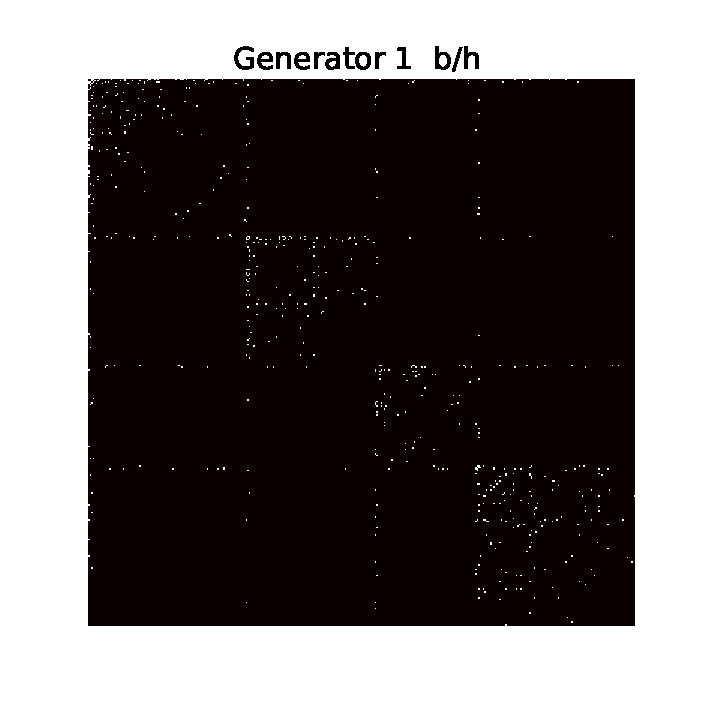
\includegraphics[scale=0.32]{img/g1}
	\endminipage
	\minipage{0.30\textwidth}
	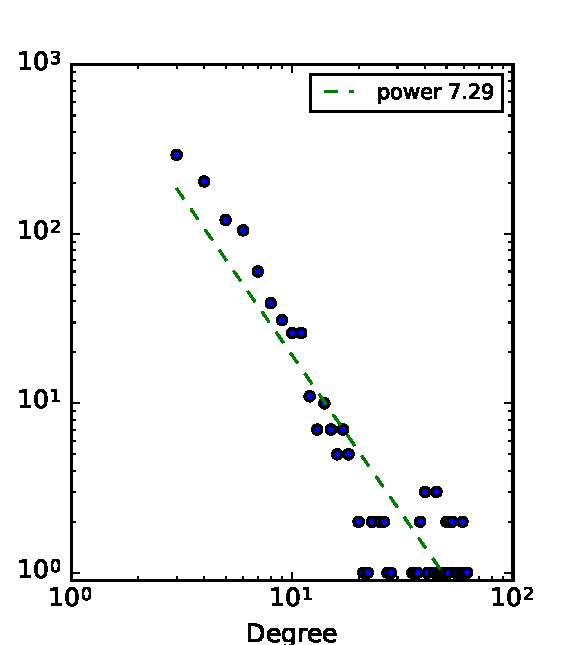
\includegraphics[scale=0.32]{img/g1_d}
	\endminipage
	\vspace{-0.4cm}
	\minipage{0.30\textwidth}
	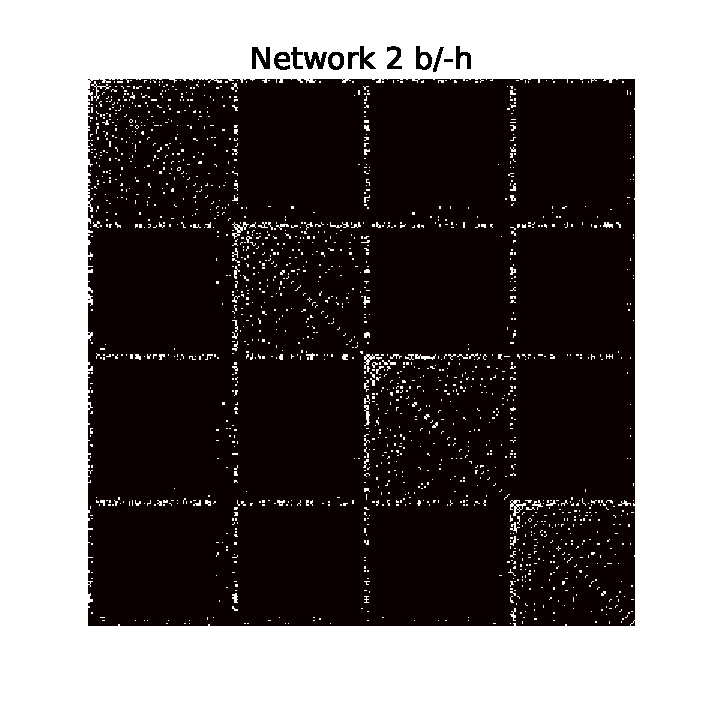
\includegraphics[scale=0.32]{img/g2}
	\endminipage
	\minipage{0.30\textwidth}
	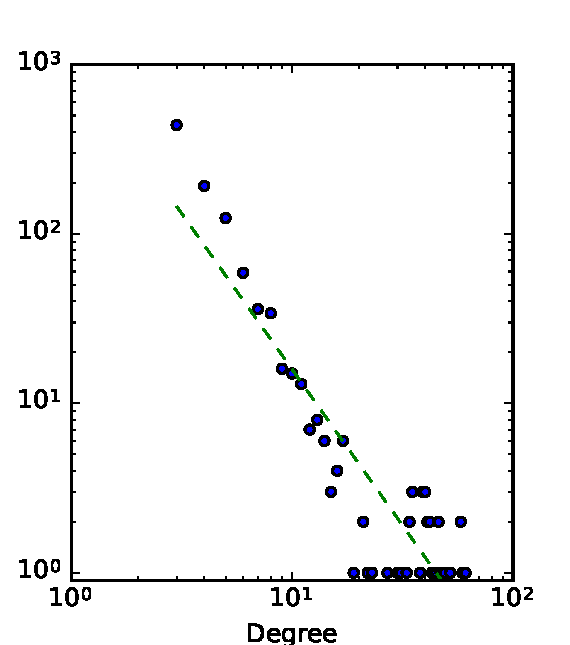
\includegraphics[scale=0.32]{img/g2_d}
	\endminipage

	%\vspace{-0.4cm}

	\minipage{0.30\textwidth}
	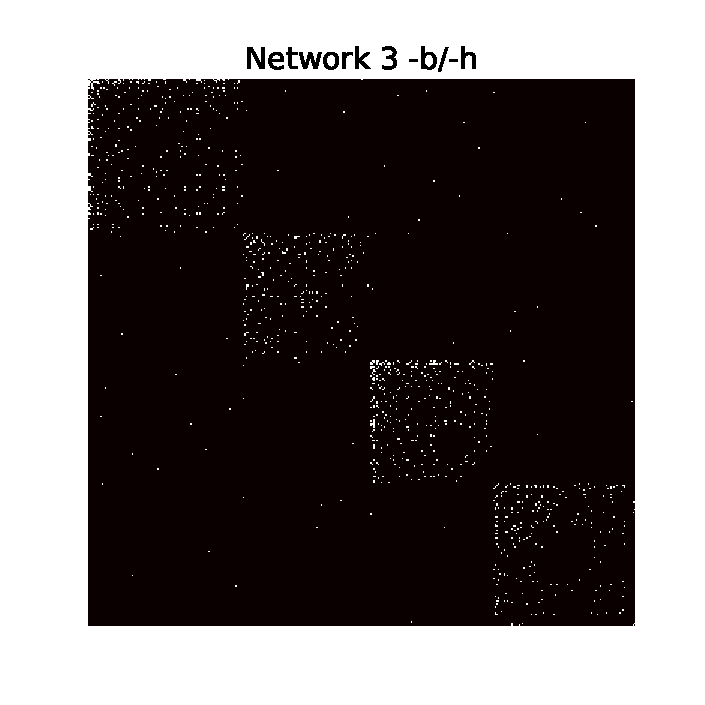
\includegraphics[scale=0.32]{img/g3}
	\endminipage
	\minipage{0.30\textwidth}
	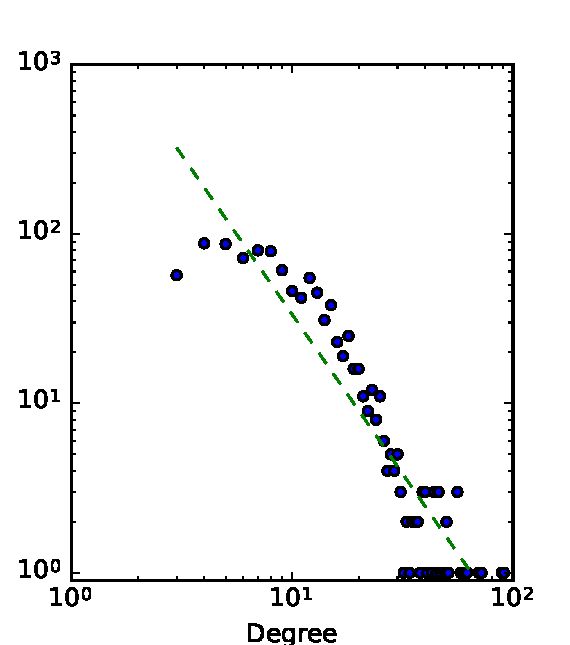
\includegraphics[scale=0.32]{img/g3_d}
	\endminipage
	\vspace{-0.4cm}
	\minipage{0.30\textwidth}
	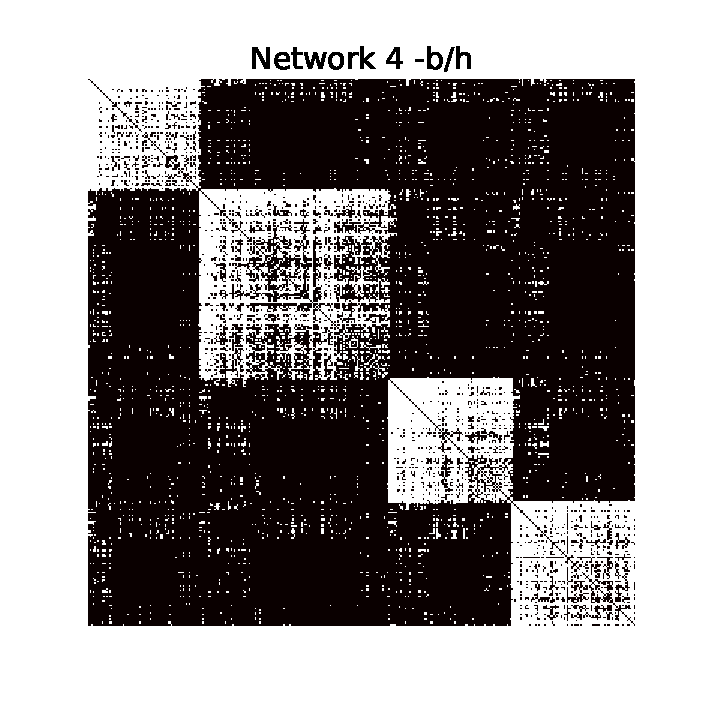
\includegraphics[scale=0.32]{img/g4}
	\endminipage
	\minipage{0.30\textwidth}
	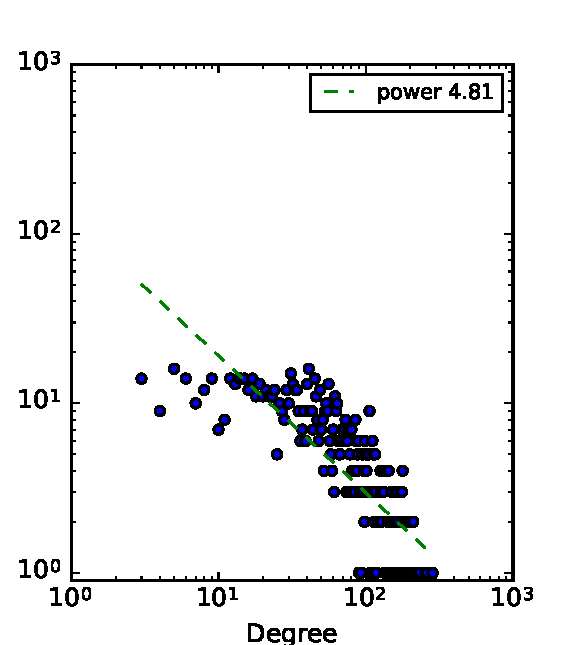
\includegraphics[scale=0.32]{img/g4_d}
	\endminipage
	
	\caption{Left subfigures represent the adjacency matrices for each of the 4 synthetic networks that we used for the prediction evaluation along with theirs respective global degree distribution in the right subplots.}
	\label{fig:synt_graph}
\end{figure}

\vspace{1cm}


\begin{figure}[h]
        \centering
        \begin{subfigure}[b]{0.480\textwidth}
            \centering
            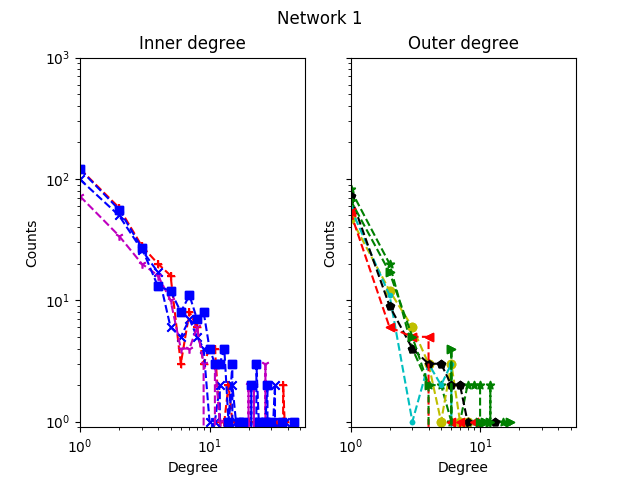
\includegraphics[width=\textwidth]{img/corpus/network1_1}
            \caption {{\small Network 1}}    
            \label{fig:mean and std of net14}
        \end{subfigure}
        \hfill
        \begin{subfigure}[b]{0.480\textwidth}  
            \centering 
            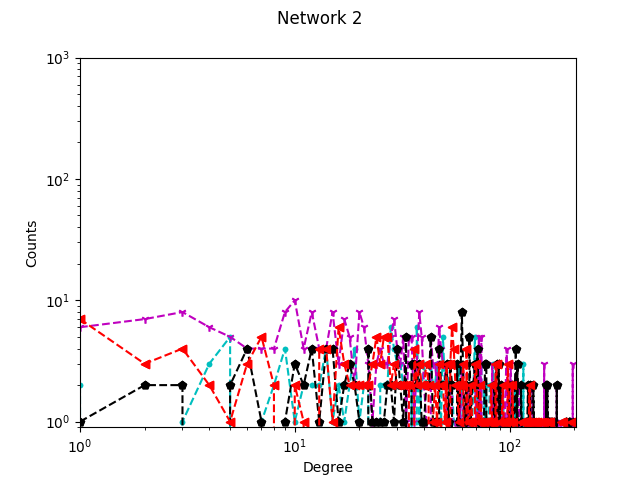
\includegraphics[width=\textwidth]{img/corpus/network2_1}
            \caption {{\small Network 2}}    
            \label{fig:mean and std of net24}
        \end{subfigure}
        \vskip\baselineskip
        \begin{subfigure}[b]{0.480\textwidth}   
            \centering 
            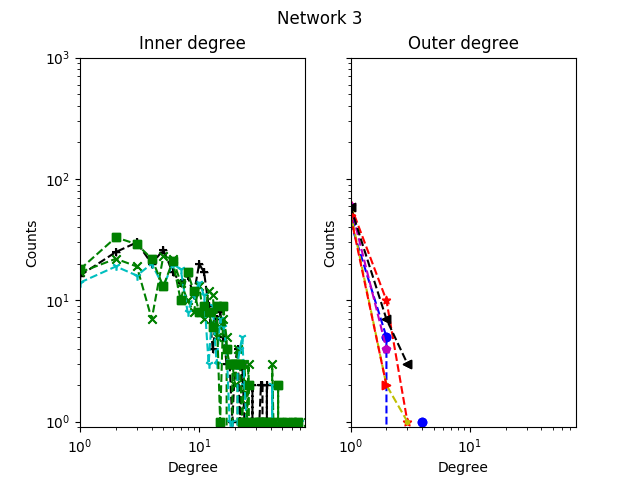
\includegraphics[width=\textwidth]{img/corpus/network3_1}
            \caption{{\small Network 3}}    
            \label{fig:mean and std of net34}
        \end{subfigure}
        \quad
        \begin{subfigure}[b]{0.480\textwidth}   
            \centering 
            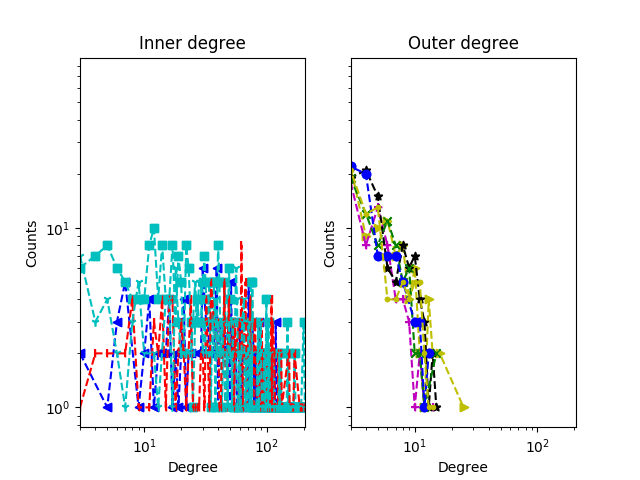
\includegraphics[width=\textwidth]{img/corpus/network4_1}
            \caption{{\small Network 4}}    
            \label{fig:mean and std of net44}
        \end{subfigure}
        \caption {Local degree distribution for the artificial networks. Inner(left) and outer(right) degree are separated.} 
	\label{fig:synt_graph_local}
\end{figure}


\begin{table}[h]
\caption{Power law goodness of fit results for characterization of global preferential attachment in synthetic networks.}
\centering
    \begin{tabular}{lrrrr}
    \hline
               &   pvalue &   alpha &   x\_min &   n\_tail \\
    \hline
     Network1 &    1.000 &   2.424 &       3 & 1000.000 \\
     Network2 &    0.971 &   2.897 &       3 & 1000.000 \\
     Network3 &    0.798 &   1.758 &       3 & 1000.000 \\
     Network4 &    0.000 &   1.354 &       3 & 1000.000 \\
    \hline
    \end{tabular}
\label{table:synt_graph}
\end{table}

\begin{table}[h]
\caption{Power law goodness of fit results for characterization of local preferential attachment in synthetic networks.}
\centering
    \begin{tabular}{lllll}
    \hline
    & pvalue          & alpha           & x\_min        & n\_tail           \\
    \hline
    Network1 & 0.9 $\pm$ 0.07  & 2.7 $\pm$ 0.1 & 1.8 $\pm$ 0.9 & 154.4 $\pm$ 83.9 \\
    Network2 & 0.9 $\pm$ 0.008 & 3.0 $\pm$ 1.2  & 1.8 $\pm$ 0.9 & 170.9 $\pm$ 66.4  \\
    Network3 & 0.8 $\pm$ 0.26 & 7.0 $\pm$ 5.8 & 1.8 $\pm$ 0.9 & 136.3 $\pm$ 94.0 \\
    Network4 & 0.6 $\pm$ 0.49    & 1.5 $\pm$ 0.1 & 1.8 $\pm$ 0.9 & 204.7 $\pm$ 53.0 \\
    \hline
    \end{tabular}
\label{table:synt_graph_local}
\end{table}


\subsection{Real networks}

We evaluate also the models on two  real networks.
The first one \footnote{available at:} is built from an online community of 1899 students from the University of California. Each node corresponds to a user and a    directed edge represents a sent message.
The second one \footnote{available at:} is an internal email communication network between employees of a mid-sized manufacturing company. Each vertex is associated  to an employee and an oriented link represents like previously a sent email.

Their adjacency matrices and global degree distribution has been reported in figure \ref{fig:real_graph}.  Table \ref{table:real_graph} summarizes some properties characteristics of these artificial and real datasets. The goodness of fit is reported in table \ref{table:real_graph}  as a reference for the global preferential attachment effect. 


%\begin{figure}[h]
%        \centering
%        \begin{subfigure}[b]{0.400\textwidth}
%            \centering
%            \includegraphics[scale=0.38]{img/corpus/fb_uc.png}
%            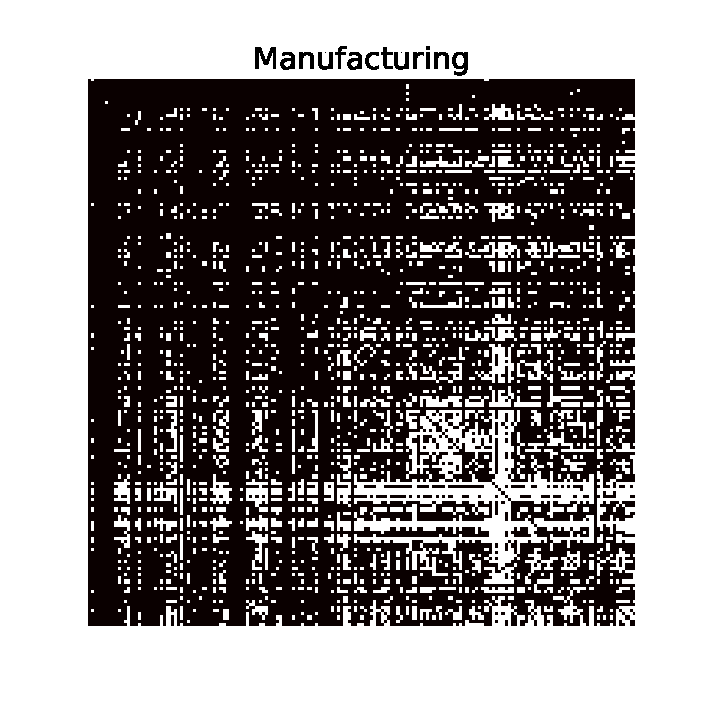
\includegraphics[scale=0.38]{img/corpus/manufacturing.png}
%            \caption {{\small Adjacency matrix}}    
%            \label{fig:mean and std of net14}
%        \end{subfigure}
%        %\hfill
%        \quad
%        \begin{subfigure}[b]{0.400\textwidth}  
%            \centering 
%            \includegraphics[scale=0.42]{img/corpus/fb_uc_d.png}
%            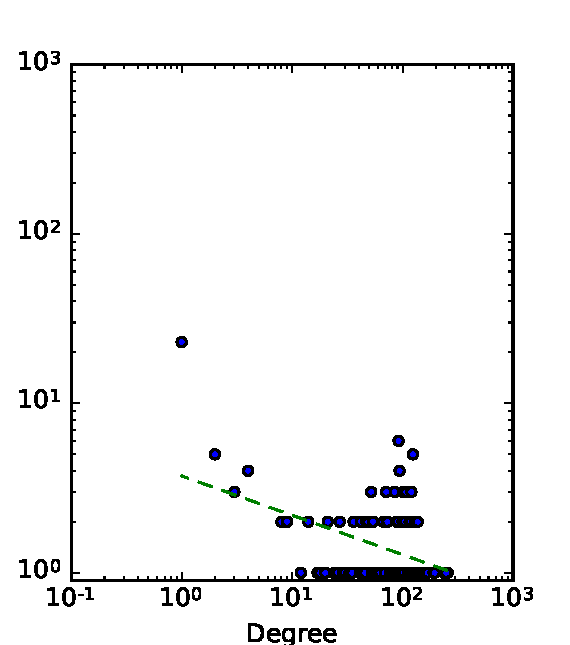
\includegraphics[scale=0.42]{img/corpus/manufacturing_d.png}
%            \caption {{\small Overall degree distributions}}    
%            \label{fig:mean and std of net24}
%        \end{subfigure}
%       \caption{Adjacency matrices (left) and global degree distributions (right) for the real networks.}
%    \label{fig:real_graph}
%\end{figure}

\begin{figure}[h]
        \centering
        \begin{subfigure}[b]{0.480\textwidth}
            \centering
            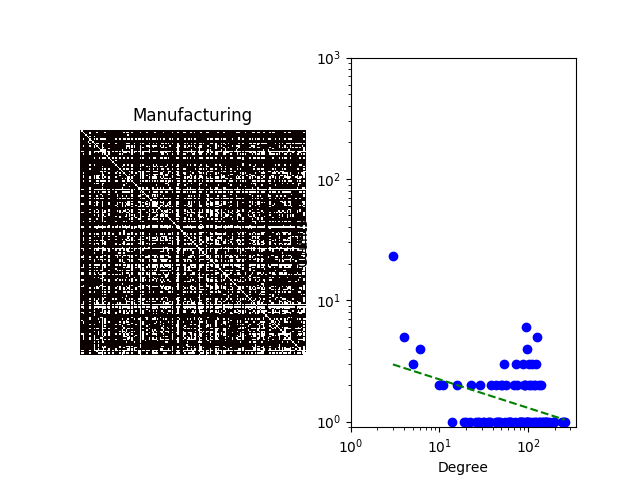
\includegraphics[width=\textwidth]{img/corpus/manufacturing_dd}
            \caption {{\small Manufacturing}}    
            \label{fig:mean and std of net14}
        \end{subfigure}
        \hfill
        \begin{subfigure}[b]{0.480\textwidth}  
            \centering 
            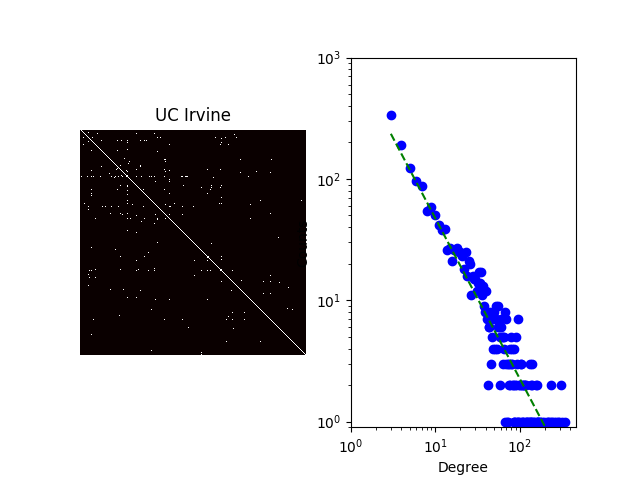
\includegraphics[width=\textwidth]{img/corpus/fb_uc_dd}
            \caption {{\small UC Irvine}}    
            \label{fig:mean and std of net24}
        \end{subfigure}
        \vskip\baselineskip
        \begin{subfigure}[b]{0.480\textwidth}   
            \centering 
            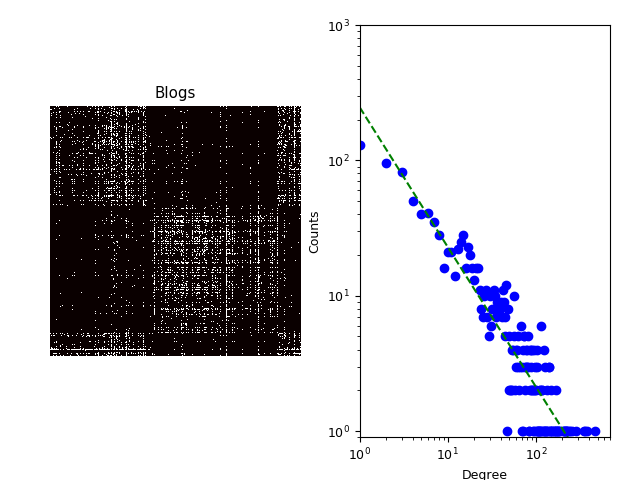
\includegraphics[width=\textwidth]{img/corpus/blogs_dd}
            \caption{{\small Blogs}}    
            \label{fig:mean and std of net34}
        \end{subfigure}
        \quad
        \begin{subfigure}[b]{0.480\textwidth}   
            \centering 
            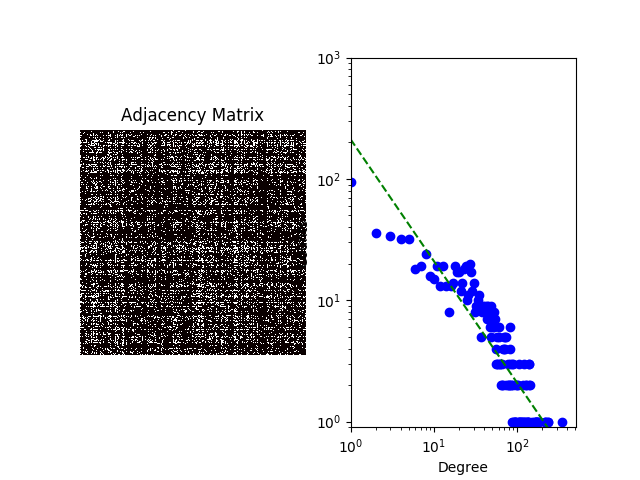
\includegraphics[width=\textwidth]{img/corpus/emaileu_dd}
            \caption{{\small Emaileu}}    
            \label{fig:mean and std of net44}
        \end{subfigure}
        \begin{subfigure}[b]{0.480\textwidth}   
            \centering 
            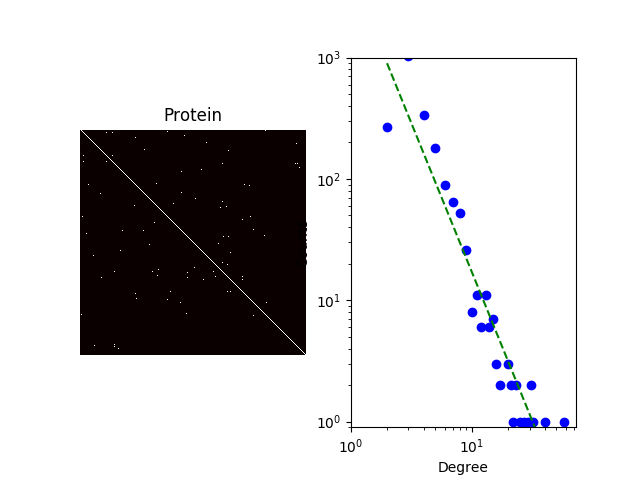
\includegraphics[width=\textwidth]{img/corpus/propro_dd}
            \caption{{\small Protein}}    
            \label{fig:mean and std of net44}
        \end{subfigure}
        %\begin{subfigure}[b]{0.480\textwidth}   
        %    \centering 
        %    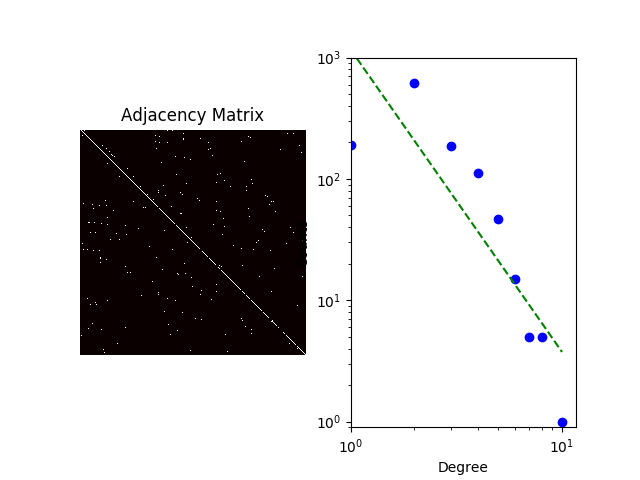
\includegraphics[width=\textwidth]{img/corpus/euroroad_dd}
        %    \caption{{\small Euroroad}}    
        %    \label{fig:mean and std of net44}
        %\end{subfigure}
	\caption{Adjacency matrices (left) and global degree distributions (right) for the real networks.}
    \label{fig:real_graph}
\end{figure}


\begin{table}
\caption{Power law goodness of fit results for characterization of global degree attachment in real networks.}
\centering
\begin{tabular}{lrrrr}
   &   pvalue &   alpha &   x\_min &   n\_tail \\
\hline
 Manufacturing &    0.000 &   1.434 &       3 &  167.000 \\
 UC Irvine     &    0.989 &   1.787 &       3 & 1899.000 \\
\hline
\end{tabular}
\label{table:real_graph}
\end{table}


\subsection{Homophily and Clustering measure }
\textcolor{red}{Temporally section, need discussion}

Here is a  table where are reported homophily (from Dancer, with the Kleinberg measure, $H_{obs} - H_{exp}$)) and clustering measure to show the correlation that exists between those measure. 

In order to highlight correlation between different properties of learning datasets (other than the burstiness). And answer the following questions: ~\\

\hspace{1cm}\textit{"Are the burstinesses effects really decorrelated from other properties (clustering, sparstity), to conclude on the fact that a model perform better than a other because of this particular properties (ie the global or local burstiness) ? (\textbf{Correlation \emph{vs} Causality}) } (the same questions holds for the impact that each properties have on each other. ) 

\begin{table}[h] 
\centering
	\caption{table:artificial networks clustering and homophily measures.}
	\begin{tabular}{lcrrr}
		\hline
		Networks   &  homophily ($H_ {obs}$ ; $\Delta_{obs - exp}$)    &  Modularity & Clustering coefff & density   \\
		\hline
		Network1  & 0.561 ;  0.08  &0.59  & 0.06 & 0.007  \\
		Network2  & 0.429 ; -0.04  &0.43  & 0.08 & 0.006 \\
		Network3  & 0.439 ; -0.03  &0.71  & 0.49 & 0.01 \\
		Network4  & 0.621 ;  0.18  &0.68  & 0.61 & 0.06 \\
		\hline
	\end{tabular}
\label{table:artificial_networks_hom}
\end{table}

\subsubsection{Comments}

\paragraph{Note on the goodness of fit results for synthetic networks:}
\begin{itemize}
    \item Network 1 to 4 have a decreasing pvalue in their overall degree distribution. Network 1 and 2 have a relatively high pvalue that suggests a high confidence in a power law fit. In the opposite, Network 4 reject the power law hypothsis strongly with a null pvalue.
    \item The analysis on local degree distribution show that network has high pvalue with a small standard deviation, while network 3 and 4 have lower pvalue and higher standard deviation which suggest that they satisfy poorly the local preferential attachment.
    \item \textcolor{red}{Put this in comparaison with homophily end sparsity ?!}
\end{itemize}


\section{$M_e$ -- Model fitted}

For each datasets described earlier, we run a MCMC inference consisting of 200 iterations to learn the posterior distribution of each the IMMSB model and ILFM, described in \ref{sec:models}. For IMMSB, concentration parameters of HDP were optimized following \cite{HDP} using vague gamma priors $\alpha_0 \sim \text{Gamma}(1,1)$ and $\gamma \sim \text{Gamma}(1,1)$. The parameter for the matrix weights were fixed to $\lambda_0=\lambda_1=0.1$. For ILFM, the IBP hyper-parameter was fixed to $\alpha=0.5$ and the weights hyper-parameter to $\sigma_w = 1$. 

The inference procedure was run under this settings in all of the 4 synthetic datasets and 2 real networks.

All our experimental platform is available online \footnote{https://github.com/dtrckd/pymake}. It is an ongoing development in order to provide a flexible way to design and run experiments and make data analysis.

\subsection{Burstiness}

In order to measure the different level of burstiness we used the models to generate full networks. (The procedure for such measure is similar than those explain in the section \ref{sec:mgmg}. Thus given the model parameters $\mathcal{M}_e = \{F ,\Phi\}$, we generate a set of 20 networks. In the next, results are averaged  with standard deviation for all those generated networks.

% Global
In figure \ref{fig:me_fit_gburst_mmsb} and \ref{fig:me_fit_gburst_ibp}, we report the global degree for generated networks for respectively IMMSB and ILFM. In Table \ref{table:global_gof}, we report the corresponding goodness of fit evaluation.



\begin{figure}[h]
        \centering
        \begin{subfigure}[b]{0.300\textwidth}
            \centering
            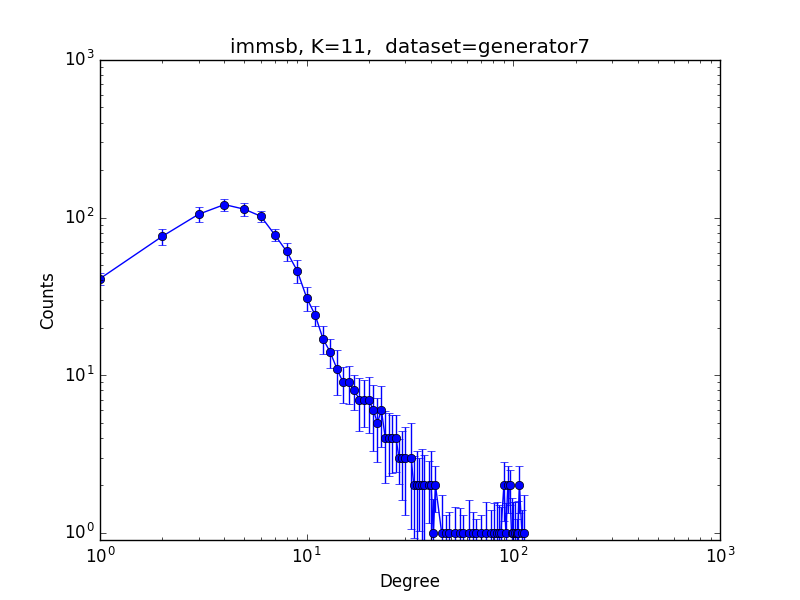
\includegraphics[width=\textwidth]{img/expe/1_mmsb/figure_1}
            \label{fig:mean and std of net14}
            \caption {{\small Network1}}    
        \end{subfigure}
        \begin{subfigure}[b]{0.300\textwidth}
            \centering
            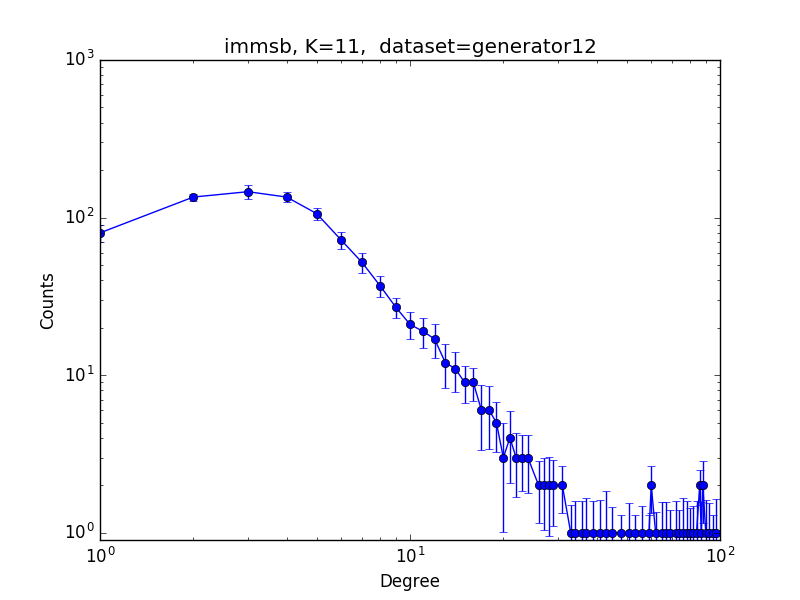
\includegraphics[width=\textwidth]{img/expe/2_mmsb/figure_1}
            \label{fig:mean and std of net14}
            \caption {{\small Network2}}    
        \end{subfigure}
        \begin{subfigure}[b]{0.300\textwidth}
            \centering
            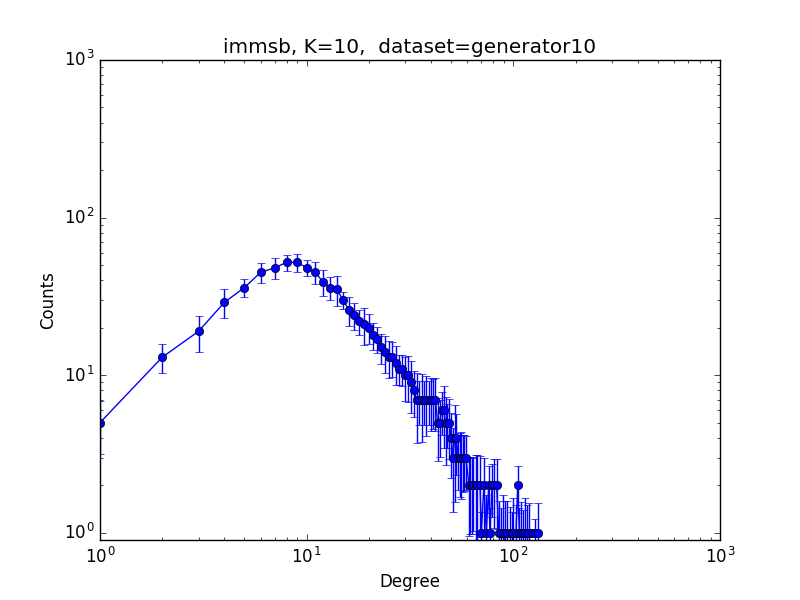
\includegraphics[width=\textwidth]{img/expe/3_mmsb/figure_1}
            \label{fig:mean and std of net14}
            \caption {{\small Network3}}    
        \end{subfigure}
        \begin{subfigure}[b]{0.300\textwidth}
            \centering
            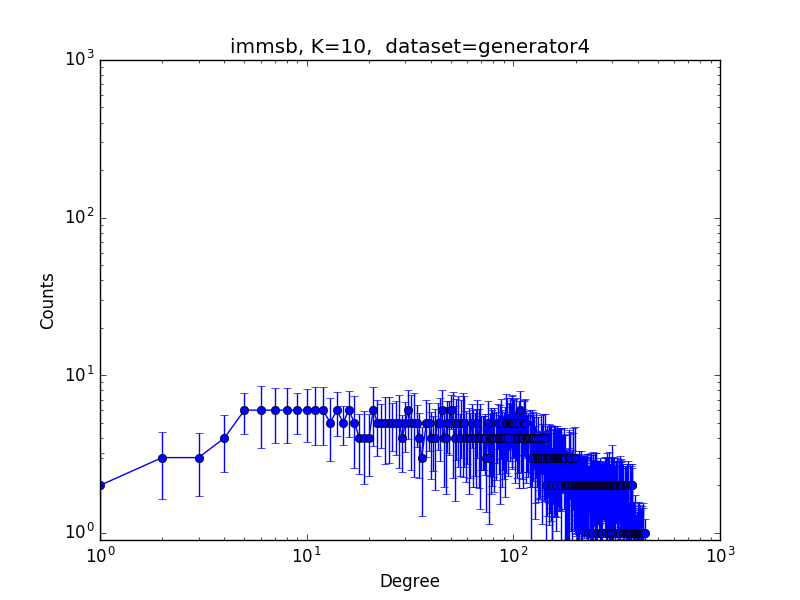
\includegraphics[width=\textwidth]{img/expe/4_mmsb/figure_1}
            \label{fig:mean and std of net14}
            \caption {{\small Network4}}    
        \end{subfigure}
        \begin{subfigure}[b]{0.300\textwidth}
            \centering
            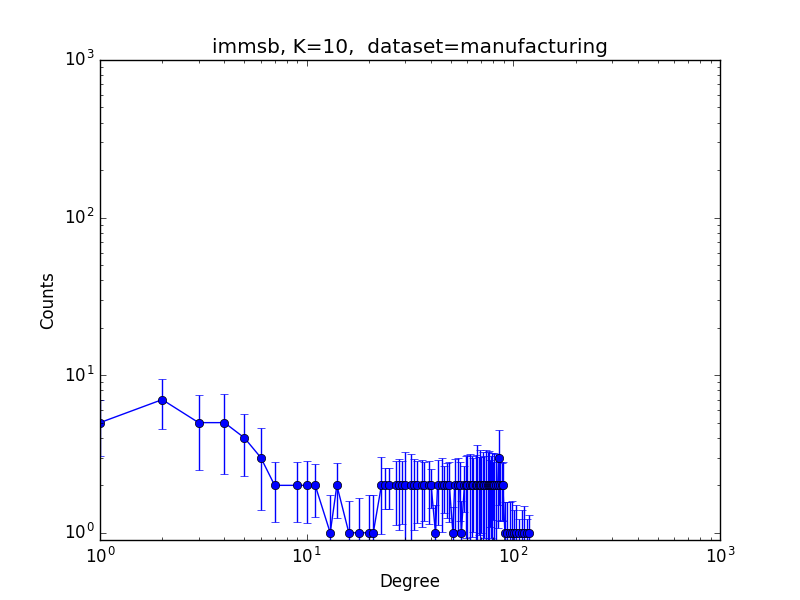
\includegraphics[width=\textwidth]{img/expe/5_mmsb/figure_1}
            \label{fig:mean and std of net14}
            \caption {{\small Manufacturing}}    
        \end{subfigure}
        \begin{subfigure}[b]{0.300\textwidth}
            \centering
            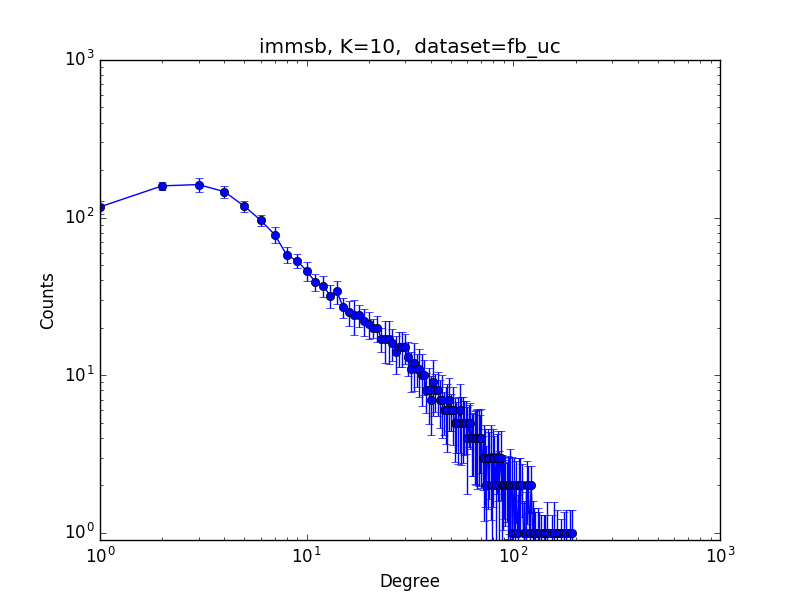
\includegraphics[width=\textwidth]{img/expe/6_mmsb/figure_1}
            \caption {{\small UC Irvine}}    
            \label{fig:mean and std of net14}
        \end{subfigure}
        %\quad
        %\hfill
        \caption{IMMSB global degree distribution in the $M_e$ settings. } 
        \label{fig:me_fit_gburst_mmsb}
\end{figure}


\begin{figure}[h]
        \centering
        \begin{subfigure}[b]{0.300\textwidth}
            \centering
            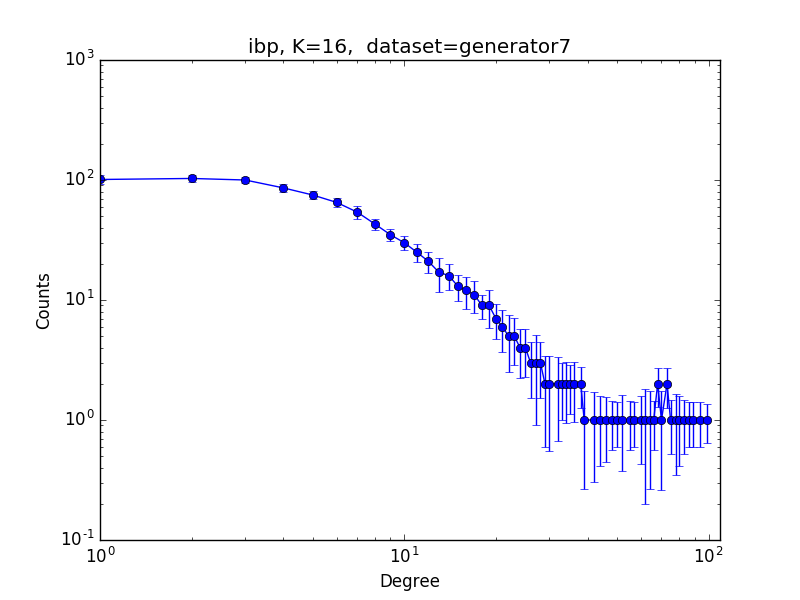
\includegraphics[width=\textwidth]{img/expe/1_ibp/figure_1}
            \label{fig:mean and std of net14}
            \caption {{\small Network1}}    
        \end{subfigure}
        \begin{subfigure}[b]{0.300\textwidth}
            \centering
            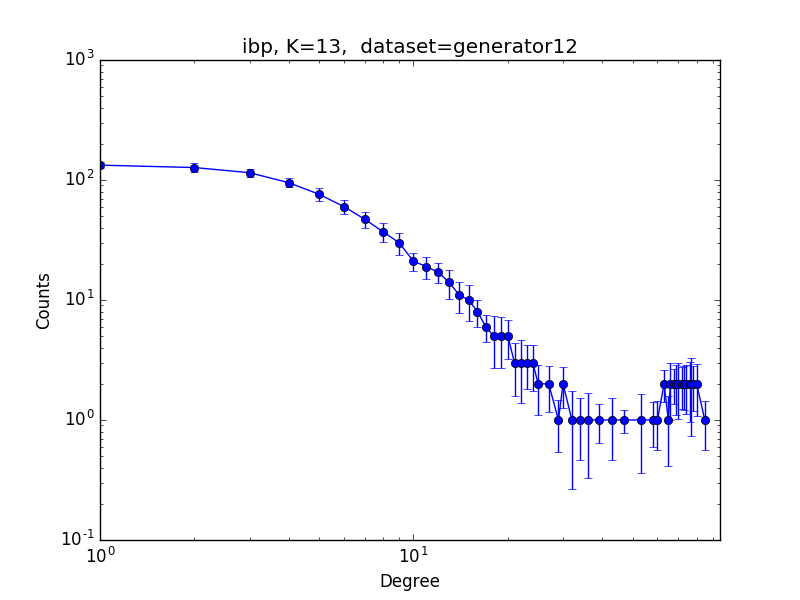
\includegraphics[width=\textwidth]{img/expe/2_ibp/figure_1}
            \label{fig:mean and std of net14}
            \caption {{\small Network2}}    
        \end{subfigure}
        \begin{subfigure}[b]{0.300\textwidth}
            \centering
            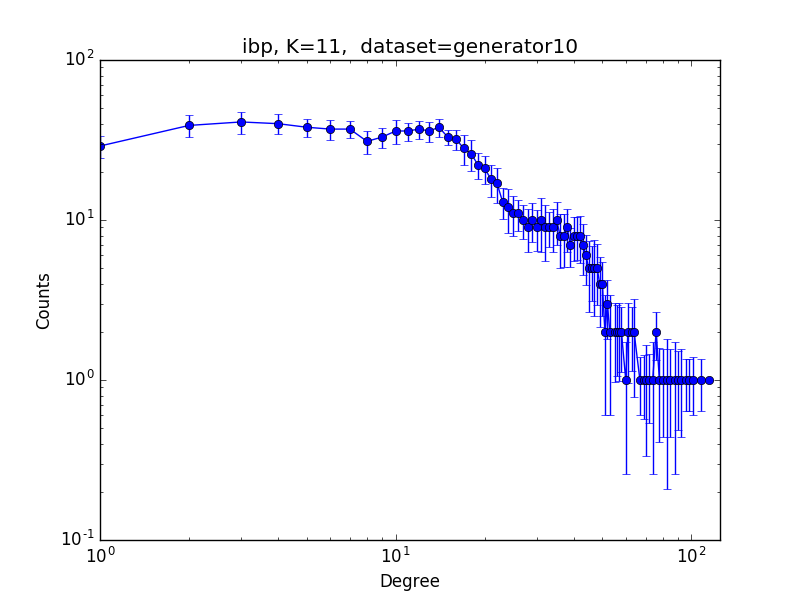
\includegraphics[width=\textwidth]{img/expe/3_ibp/figure_1}
            \label{fig:mean and std of net14}
            \caption {{\small Network3}}    
        \end{subfigure}
        \begin{subfigure}[b]{0.300\textwidth}
            \centering
            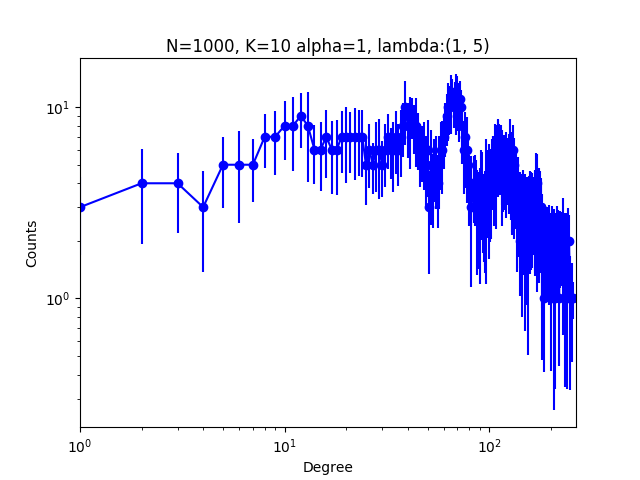
\includegraphics[width=\textwidth]{img/expe/4_ibp/figure_1}
            \label{fig:mean and std of net14}
            \caption {{\small Network4}}    
        \end{subfigure}
        \begin{subfigure}[b]{0.300\textwidth}
            \centering
            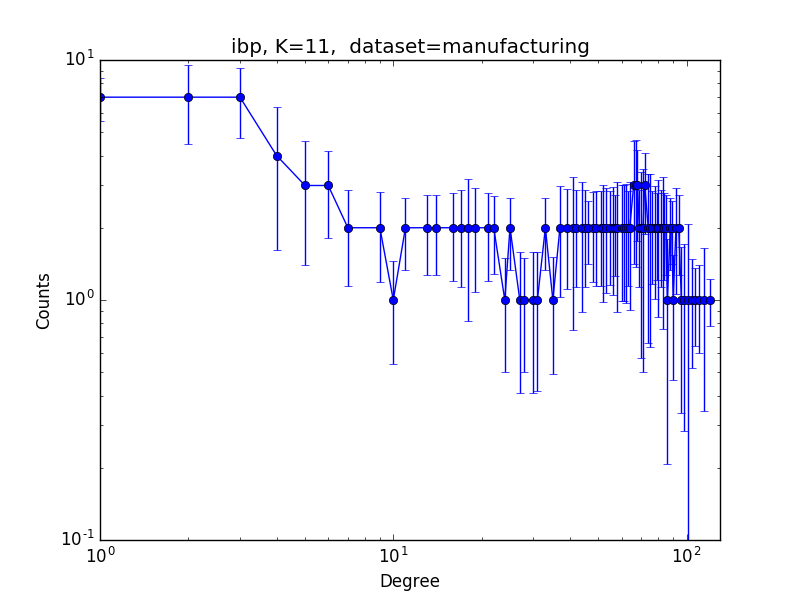
\includegraphics[width=\textwidth]{img/expe/5_ibp/figure_1}
            \label{fig:mean and std of net14}
            \caption {{\small Manufacturing}}    
        \end{subfigure}
        \begin{subfigure}[b]{0.300\textwidth}
            \centering
            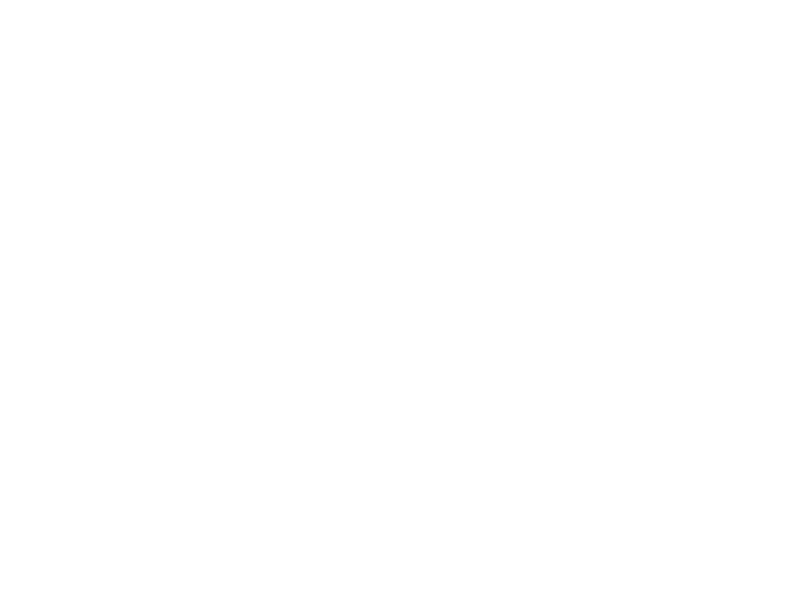
\includegraphics[width=\textwidth]{img/expe/6_ibp/figure_1}
            \caption {{\small UC Irvine}}    
            \label{fig:mean and std of net14}
        \end{subfigure}
        %\quad
        %\hfill
        \caption{ILFM global degree distribution in the $M_e$ settings. } 
\end{figure}


\begin{table}
    \caption{Power law Goodness of fit for the global preferential attachment effect.}
\centering
    \begin{tabular}{lllll}
    \hline
        \textbf{IMMSB} & pvalue          & alpha           & x\_min          & n\_tail           \\
    \hline
    Network1     & 0.907 $\pm$ 0.11 & 1.396 $\pm$ 0.004 & 1.0 $\pm$ 0.0    & 990.1 $\pm$ 3.1  \\
    Network2     & 1.0 $\pm$ 0.0     & 1.452 $\pm$ 0.005 & 1.0 $\pm$ 0.0    & 974.4 $\pm$ 4.9  \\
    Network3     & 0.0 $\pm$ 0.0     & 1.294 $\pm$ 0.001 & 1.0 $\pm$ 0.0    & 999.0 $\pm$ 0.9 \\
    Network4     & 0.0 $\pm$ 0.0     & 1.203 $\pm$ 0.025 & 1.25 $\pm$ 0.5 & 999.1 $\pm$ 0.7 \\
    Manufacturing & 0.006 $\pm$ 0.01 & 1.244 $\pm$ 0.002 & 1.0 $\pm$ 0.0    & 165.3 $\pm$ 1.3 \\
    UC Irvine     & 1.0 $\pm$ 0.0     & 1.348 $\pm$ 0.002 & 1.0 $\pm$ 0.0    & 1852.7 $\pm$ 5.7 \\
    \hline
    \end{tabular}

    \begin{tabular}{lllll}
    \hline
        \textbf{ILFM} & pvalue          & alpha           & x\_min       & n\_tail           \\
    \hline
    Network1     & 1.0 $\pm$ 0.0     & 1.4 $\pm$ 0.003 & 1.0 $\pm$ 0.0 & 919.5 $\pm$ 5.9 \\
    Network2     & 1.0 $\pm$ 0.0     & 1.4 $\pm$ 0.004 & 1.0 $\pm$ 0.0 & 893.7 $\pm$ 7.1  \\
    Network3     & 0.01 $\pm$ 0.02  & 1.3 $\pm$ 0.002 & 1.0 $\pm$ 0.0 & 982.7 $\pm$ 3.6 \\
    Network4     & 0.0 $\pm$ 0.0     & 1.2 $\pm$ 0.018 & 1.1 $\pm$ 0.3 & 998.4 $\pm$ 0.9 \\
    Manufacturing & 0.018 $\pm$ 0.01 & 1.2 $\pm$ 0.002 & 1.0 $\pm$ 0.0 & 164.2 $\pm$ 1.4 \\
    UC Irvine     & 1.0 $\pm$ 0.0     & 1.3 $\pm$ 0.002 & 1.0 $\pm$ 0.0 & 1798.3 $\pm$ 8.2 \\
    \hline
    \end{tabular}
    \label{table:global_gof}
\end{table}



% Local
In figure \ref{fig:me_fit_lburst_mmsb} and \ref{fig:me_fit_lburst_ibp}, we report the local degree for generated networks for respectively IMMSB and ILFM. In Table \ref{table:local_gof}, we report the corresponding goodness of fit evaluation. \underline{Note that the pvalue reported here, are the averaged of all} classes.


\textcolor{red}{here comment...} ~\\
\textcolor{red}{x\_min could be removed from table, I explains earlier how I choose it.}


\begin{figure}[h]
        \centering
        \begin{subfigure}[b]{0.300\textwidth}
            \centering
            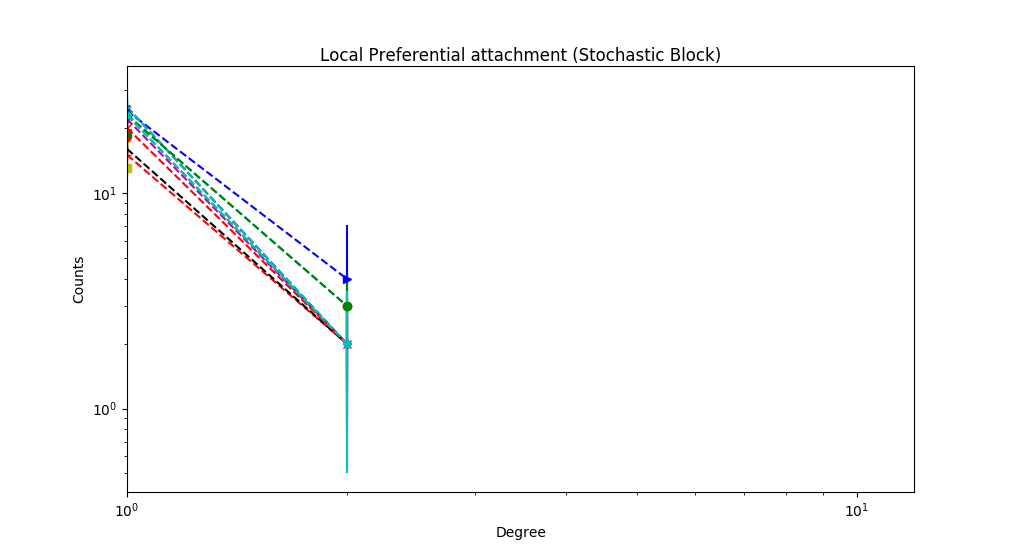
\includegraphics[width=\textwidth]{img/expe/1_mmsb/figure_2}
            \label{fig:mean and std of net14}
            \caption {{\small Network1}}    
        \end{subfigure}
        \begin{subfigure}[b]{0.300\textwidth}
            \centering
            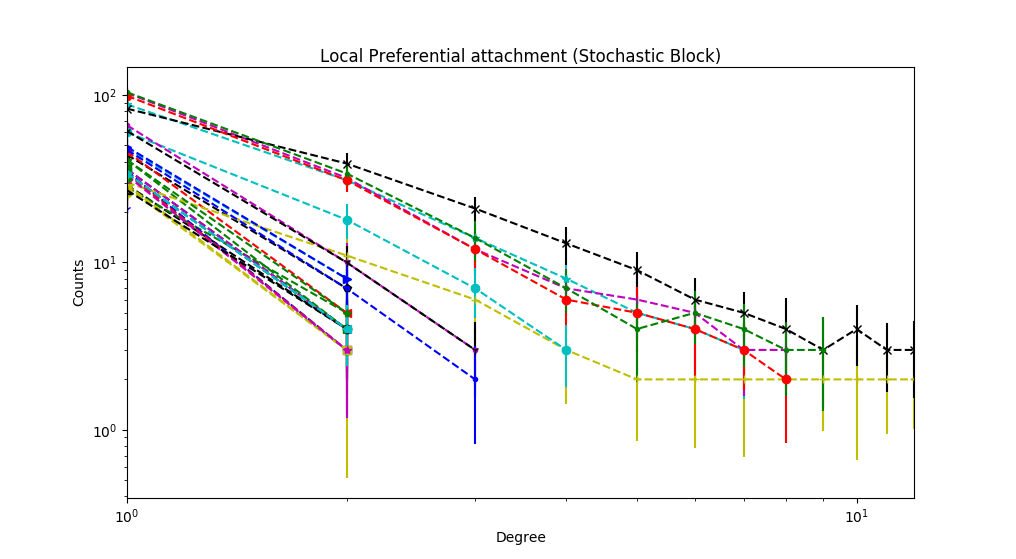
\includegraphics[width=\textwidth]{img/expe/2_mmsb/figure_2}
            \label{fig:mean and std of net14}
            \caption {{\small Network2}}    
        \end{subfigure}
        \begin{subfigure}[b]{0.300\textwidth}
            \centering
            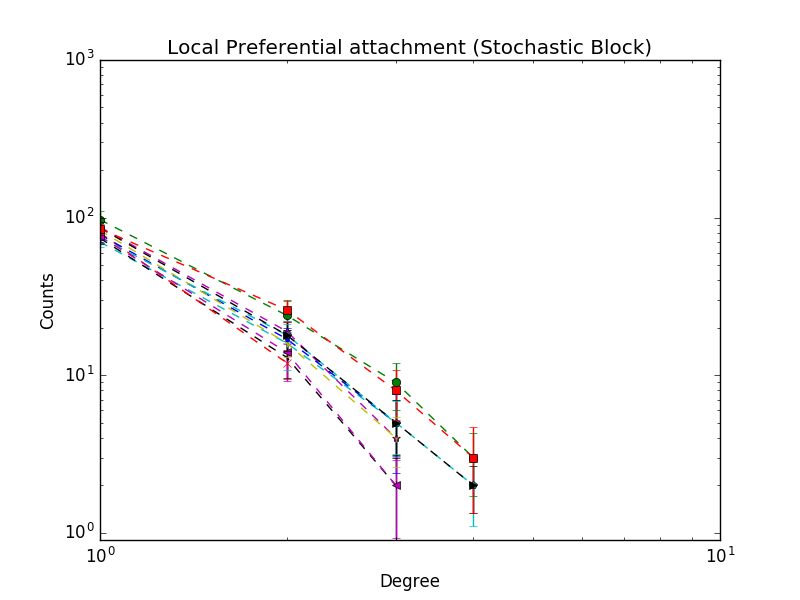
\includegraphics[width=\textwidth]{img/expe/3_mmsb/figure_2}
            \label{fig:mean and std of net14}
            \caption {{\small Network3}}    
        \end{subfigure}
        \begin{subfigure}[b]{0.300\textwidth}
            \centering
            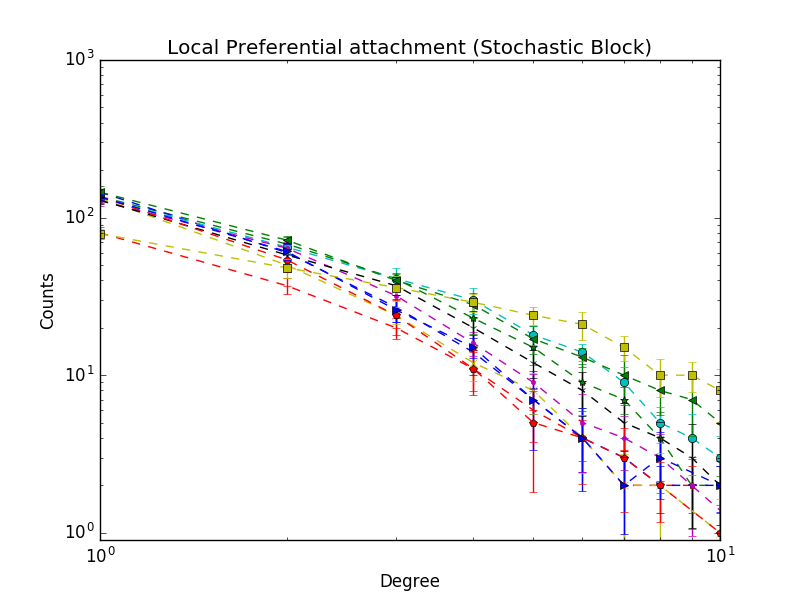
\includegraphics[width=\textwidth]{img/expe/4_mmsb/figure_2}
            \label{fig:mean and std of net14}
            \caption {{\small Network4}}    
        \end{subfigure}
        \begin{subfigure}[b]{0.300\textwidth}
            \centering
            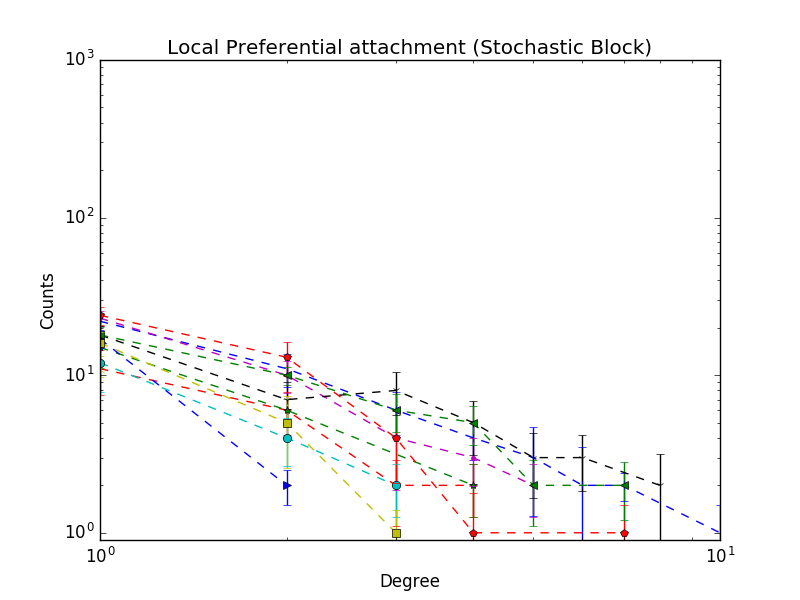
\includegraphics[width=\textwidth]{img/expe/5_mmsb/figure_2}
            \label{fig:mean and std of net14}
            \caption {{\small Manufacturing}}    
        \end{subfigure}
        \begin{subfigure}[b]{0.300\textwidth}
            \centering
            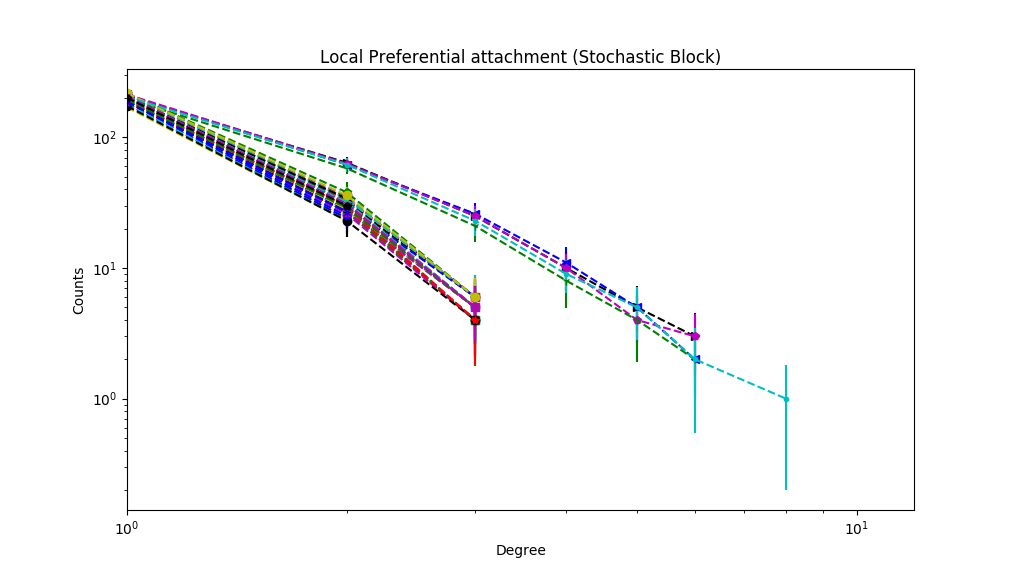
\includegraphics[width=\textwidth]{img/expe/6_mmsb/figure_2}
            \caption {{\small UC Irvine}}    
            \label{fig:mean and std of net14}
        \end{subfigure}
        %\quad
        %\hfill
        \caption{IMMSB Local degree distribution in the $M_e$ settings. } 
\end{figure}


\begin{figure}[h]
        \centering
        \begin{subfigure}[b]{0.300\textwidth}
            \centering
            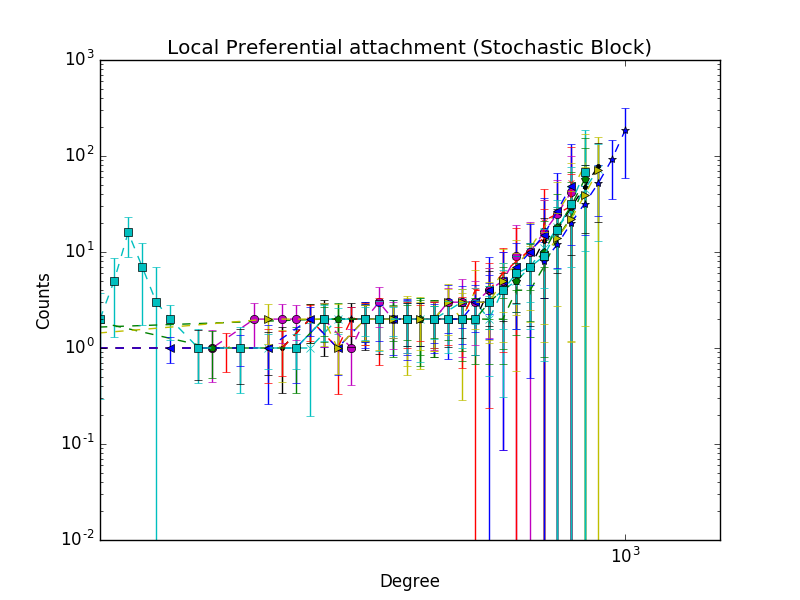
\includegraphics[width=\textwidth]{img/expe/1_ibp/figure_2}
            \label{fig:mean and std of net14}
            \caption {{\small Network1}}    
        \end{subfigure}
        \begin{subfigure}[b]{0.300\textwidth}
            \centering
            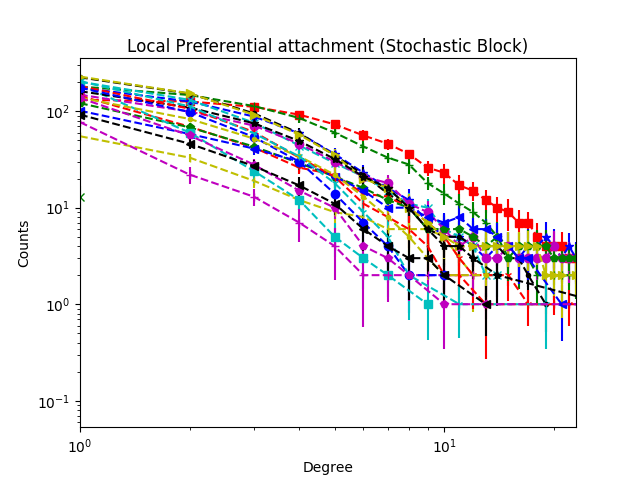
\includegraphics[width=\textwidth]{img/expe/2_ibp/figure_2}
            \label{fig:mean and std of net14}
            \caption {{\small Network2}}    
        \end{subfigure}
        \begin{subfigure}[b]{0.300\textwidth}
            \centering
            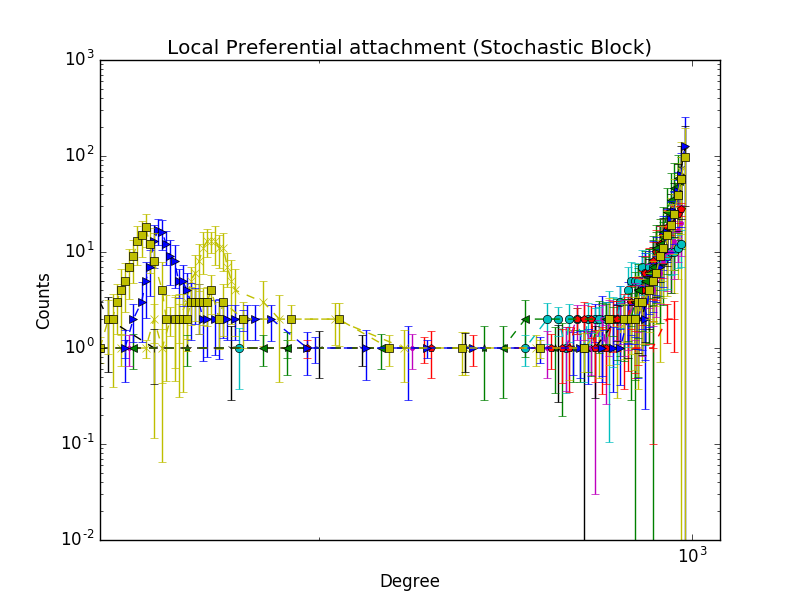
\includegraphics[width=\textwidth]{img/expe/3_ibp/figure_2}
            \label{fig:mean and std of net14}
            \caption {{\small Network3}}    
        \end{subfigure}
        \begin{subfigure}[b]{0.300\textwidth}
            \centering
            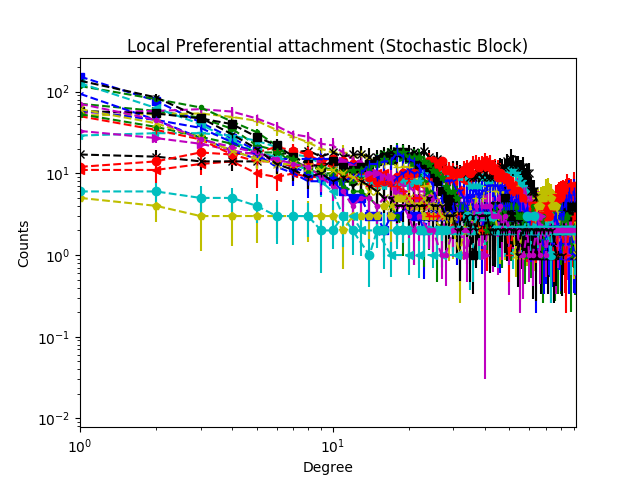
\includegraphics[width=\textwidth]{img/expe/4_ibp/figure_2}
            \label{fig:mean and std of net14}
            \caption {{\small Network4}}    
        \end{subfigure}
        \begin{subfigure}[b]{0.300\textwidth}
            \centering
            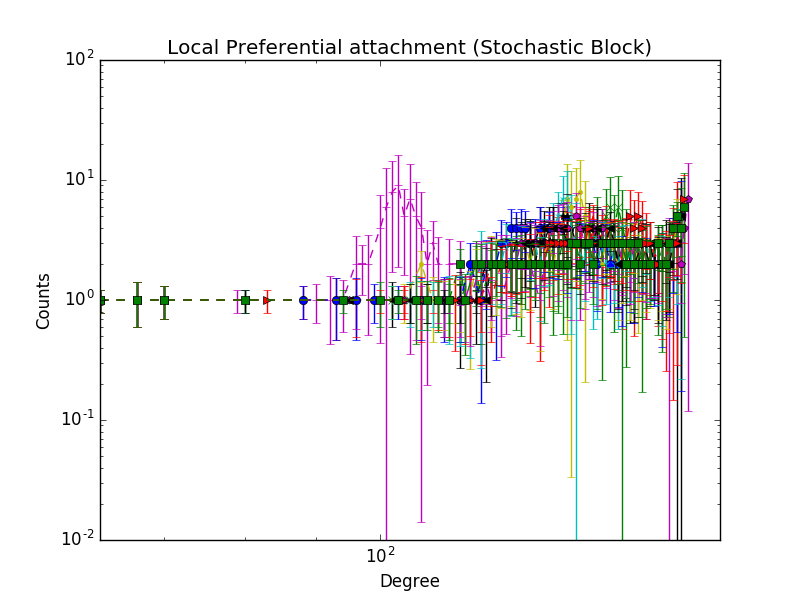
\includegraphics[width=\textwidth]{img/expe/5_ibp/figure_2}
            \label{fig:mean and std of net14}
            \caption {{\small Manufacturing}}    
        \end{subfigure}
        \begin{subfigure}[b]{0.300\textwidth}
            \centering
            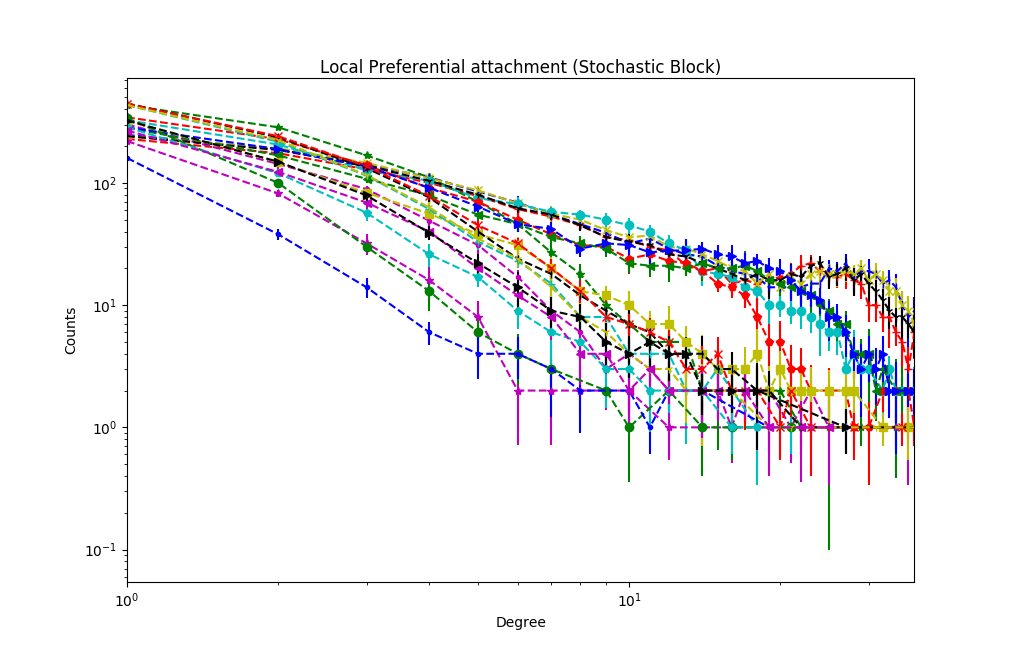
\includegraphics[width=\textwidth]{img/expe/6_ibp/figure_2}
            \label{fig:mean and std of net14}
            \caption {{\small UC Irvine}}    
        \end{subfigure}
        %\quad
        %\hfill
        \caption{ILFM Local degree distribution in the $M_e$ settings. } 
        \label{fig:me_fit_lburst_ibp}
\end{figure}



\begin{table}
    \caption{Power law Goodness of fit for the local preferential attachment effect.}
\centering
    \begin{tabular}{lllll}                                                                                    
    \hline                                                                
        \textbf{IMMSB}  & pvalue         & alpha           & x\_min          & n\_tail             \\            
    \hline                                                                                                    
    Network1     & 1.0 $\pm$ 0.0    & 7.433 $\pm$ 2.2 & 1.0 $\pm$ 0.0    & 53.737 $\pm$ 9.8   \\
    Network2     & 1.0 $\pm$ 0.0    & 1 $\pm$ 0.0    & 1.0 $\pm$ 0.0    & 41.895 $\pm$ 11.2  \\                             
    Network3     & 1.0 $\pm$ 0.0    & 4.074 $\pm$ 0.7 & 1.0 $\pm$ 0.0    & 112.143 $\pm$ 18.5 \\                
    Network4     & 1.0 $\pm$ 0.0    & 1.957 $\pm$ 0.2 & 1.0 $\pm$ 0.0    & 316.095 $\pm$ 69.5 \\
    Manufacturing & 0.55 $\pm$ 0.5 & 1.242 $\pm$ 1.1 & 0.55 $\pm$ 0.4 & 31.4 $\pm$ 14.644    \\              
    UC Irvine     & 1.0 $\pm$ 0.0    & 5.213 $\pm$ 0.9 & 1.0 $\pm$ 0.0    & 242.0 $\pm$ 26.1   \\                
    \hline                                                                
    \end{tabular}    

    \begin{tabular}{lllll}
    \hline
        \textbf{ILFM} & pvalue          & alpha           & x\_min           & n\_tail              \\
    \hline
    Network1     & 1.0 $\pm$ 0.0     & 1.93 $\pm$ 0.3  & 1.0 $\pm$ 0.0     & 325.7 $\pm$ 154.9 \\
    Network2     & 0.952 $\pm$ 0.2 & 1.76 $\pm$ 0.5 & 0.9 $\pm$ 0.2 & 423.8 $\pm$ 210.1  \\
    Network3     & 0.957 $\pm$ 0.2 & 1.58 $\pm$ 0.3 & 1.0 $\pm$ 0.0     & 587.0 $\pm$ 252.2 \\
    Network4     & 0.698 $\pm$ 0.4 & 1.33 $\pm$ 0.1 & 1.0 $\pm$ 0.0     & 632.9 $\pm$ 200.1  \\
    Manufacturing & 0.69 $\pm$ 0.3   & 1.40 $\pm$ 0.2 & 1.0 $\pm$ 0.0     & 92.0 $\pm$ 26.5     \\
    UC Irvine     & 1.0 $\pm$ 0.0     & 1.87 $\pm$ 0.4   & 1.0 $\pm$ 0.0     & 994.3 $\pm$ 408.8 \\
    \hline
    \end{tabular}
\label{table:local_gof}
\end{table}

\subsubsection{Comments}

\textcolor{red}{here comment...} 

\subsection{Homophily}

%We evaluate in this section the behaviour of homophily of models according to both, the natural and the latent similarity, reported respectively in tables \ref{table:homo_natural} and \ref{table:homo_latent}. Those results are obtained by computing the Pearson correlation coefficient between a random adjacency matrix and a similarity matrix matrix as defined in \ref{sec_homophily} from a model (either IMMSB or ILFM). Each of these coefficient is averaged an basis on 20 networks generated from the fitted models.

%Firstly, we can notice that the results are stable since the standard deviation is not significant for all experiments. Secondly those results illustrate the fact that both models are homophilic under the natural similarity with a positive correlation in all networks,  and not under the latent similarity with a correlation coefficient near to 0 and oscillating between positive and negative value (Note that this last fact depend on the initialization and the seed of the models).

%%%% correlation betewwen edges and similarity
%\begin{table}
%\caption{Correlation between the natural similarity matrix and adjacency matrix for IMMSB and ILFM.}
%\centering
%    \begin{tabular}{lll}
%    \hline
%    & IMMSB   & ILFM  \\
%    \hline
%    Network1     & 0.23 $\pm$ 0.004  & 0.135 $\pm$ 0.001      \\
%    Network2     & 0.225 $\pm$ 0.005 & 0.112 $\pm$ 0.001      \\
%    Network3     & 0.186 $\pm$ 0.002 & 0.165 $\pm$ 0.001      \\
%    Network4     & 0.385 $\pm$ 0.001 & 0.443 $\pm$ 0.0        \\
%    Manufacturing & 0.661 $\pm$ 0.003 & 0.583 $\pm$ 0.002      \\
%    UC Irvine     & 0.21 $\pm$ 0.002  & 0.129 $\pm$ 0.001      \\
%    \hline
%    \end{tabular}
%\label{table:homo_natural}
%\end{table}
%
%
%\begin{table}
%    \caption{Correlation between the latent similarity matrix and adjacency matrix for IMMSB and ILFM.}
%    \begin{tabular}{lll}
%    \hline
%    & ILFM  & IMMSB \\
%    \hline
%    Network1     & 0.021 $\pm$ 0.001  & -0.035 $\pm$ 0.001      \\
%    Network2     & -0.007 $\pm$ 0.001 & -0.051 $\pm$ 0.001      \\
%    Network3     & 0.012 $\pm$ 0.001  & 0.002 $\pm$ 0.001       \\
%    Network4     & 0.141 $\pm$ 0.001  & 0.056 $\pm$ 0.001       \\
%    Manufacturing & 0.11 $\pm$ 0.003   & 0.073 $\pm$ 0.004       \\
%    UC Irvine     & 0.148 $\pm$ 0.002  & -0.063 $\pm$ 0.0        \\
%    \hline
%    \end{tabular}
%\label{table:homo_latent}
%\end{table}


We evaluate in this section the behaviour of homophily of models according to both, the natural and the latent similarity.

In table  \ref{table:homo_latent} we compute the Pearson correlation for the homophily measure. Note that this coefficient for the natural similarity is always equal to one.

\begin{table}
    \caption{Correlation between the latent similarity matrix and the predictive likelihood for IMMSB and ILFM.}
    \label{table:homo_conting}

    to come...


\end{table}

\begin{table}
    \caption{Correlation between the latent similarity matrix and the predictive likelihood for IMMSB and ILFM.}
    \begin{tabular}{lll}
    \hline
%    & ILFM  & IMMSB \\
    \hline
    Network 1     & 0.082 &  -0.126   \\
    Network 2     & 0.001     &  -0.116   \\
    Network 3     & 0.114     &  0.123    \\
    Network 4     & 0.076     &  0.009    \\
    Manufacturing & 0.384     &  -0.011   \\
    UC Irvine     & 0.286     &  -0.213   \\
    \hline
    \label{table:homo_latent}
    \end{tabular}
\end{table}


\subsubsection{Comments}
\textcolor{red}{here comment...} 



\subsection{Prediction Performance}
In order to evaluate the  prediction performance of the models, we build a training set and a testing set from the original datasets. In order to achieve this, we generate a random mask consisting of 20 percent of the size of the adjacency matrix. This mask is used a our testing set, while the 80 remaining percent are used as a training set. The results for the prediction evaluation are reported in i) the AUC-ROC measures in figure \ref{fig:auc}, and ii) in the precision/recall results in table \ref{table:unbalanced}.
Each prediction results were averaged on 10 repetitions, and results were found to be stable regarding on the random  initialization and the stochastic optimization procedure. 

% Debug 12 / MASK all

% K = 5

\begin{table*}[h] 
\caption{Predictive Performance for Synthetic datasets}
	\begin{minipage}[h]{0.45\linewidth} 
      \resizebox{\textwidth}{!}{  
K = 5\hspace{5pt}
\begin{tabular}{llllll}
\hline
 IMMSB   &   global &   precision &   recall & $f_1$ &    K-\ensuremath{>} \\
\hline
Network1        &    0.990 &       0.029 &    0.032 & 0.030 & 5.3 $\pm$ 0.4 \\
Network2       &    0.992 &       0.032 &    0.034 &  0.032 & 5.8 $\pm$ 1.1 \\
Network3        &    0.979 &       0.031 &    0.034 & 0.032 & 5.1 $\pm$ 0.3     \\
Network4       &    0.887 &       0.151 &    0.192 &  0.170 & 5.4 $\pm$ 0.4 \\

\hline
\end{tabular}
        }
\end{minipage}
\hspace{0.8cm}
\begin{minipage}[h]{0.45\linewidth}
      \resizebox{\textwidth}{!}{  
\begin{tabular}{llllll}
\hline
  ILFM & global &   precision &   recall &   $f_1$ &   K-\ensuremath{>} \\
\hline
Network1      &    0.990 &       0.051 &    0.053 &  0.053 &  13.4 $\pm$ 0.8    \\
Network2     &    0.992 &       0.044 &    0.045 &   0.044 &  14.0 $\pm$ 2.0    \\
Network3      &    0.982 &       0.114 &    0.116 &  0.121 &  10.0 $\pm$ 2.1 \\
Network4     &    0.926 &       0.389 &    0.393 &   0.390 &  7.2 $\pm$ 1.6     \\

\hline
\end{tabular}
    }
\end{minipage}

% K = 10

	\begin{minipage}[h]{0.45\linewidth} 
      \resizebox{\textwidth}{!}{  
K = 10
\begin{tabular}{llllll}
Network1       &    0.990 &       0.044 &    0.046 &  0.042 & 10.8 $\pm$ 0.6 \\
Network2      &    0.992 &       0.039 &    0.045 &   0.039 & 10.8 $\pm$ 0.6 \\
Network3       &    0.979 &       0.030 &    0.035 &  0.032 & 11.0 $\pm$ 1.0 \\
Network4      &    0.897 &       0.202 &    0.238 &   0.206 & 10.4 $\pm$ 0.8 \\

\hline
\end{tabular}
    }
\end{minipage}
\hspace{0.8cm}
\begin{minipage}[h]{0.45\linewidth}
      \resizebox{\textwidth}{!}{  
\begin{tabular}{llllll}
Network1      &    0.990 &       0.049 &    0.053 &  0.055 &  17.2 $\pm$ 2.8 \\
Network2     &    0.992 &       0.047 &    0.051 &   0.052 &  17.2 $\pm$ 2.1 \\
Network3      &    0.982 &       0.132 &    0.132 &  0.137 &  12.2 $\pm$ 2.0 \\
Network4     &    0.934 &       0.448 &    0.447 &   0.463 &  9.2 $\pm$ 1.2 \\

\hline
\end{tabular}
    }
\end{minipage}

% K = 15

	\begin{minipage}[h]{0.45\linewidth} 
      \resizebox{\textwidth}{!}{  
K = 15
\begin{tabular}{lrrrrr}
Network1        &    0.990 &       0.038 &    0.041 &    0.040 &  15.6 $\pm$ 1.0 \\
Network2       &    0.992 &       0.036 &    0.038 &     0.037 &  16.0 $\pm$ 0.8 \\
Network3        &    0.979 &       0.029 &    0.032 &    0.033 &  15.5 $\pm$ 0.5 \\
Network4       &    0.898 &       0.207 &    0.245 &     0.229 &  15.5 $\pm$ 0.8 \\

\hline
\end{tabular}
    }
\end{minipage}
\hspace{0.8cm}
\begin{minipage}[h]{0.45\linewidth}
      \resizebox{\textwidth}{!}{  
\begin{tabular}{lrrrrr}
Network1      &    0.990 &       0.050 &    0.053 &  0.007 &      20.6 $\pm$ 2.1 \\
Network2     &    0.992 &       0.049 &    0.055 &   0.049 &      21.2 $\pm$ 2.1 \\
Network3      &    0.983 &       0.164 &    0.166 &  0.164 &      17.2 $\pm$ 1.3 \\
Network4     &    0.939 &       0.499 &    0.501 &   0.499 &      14.8 $\pm$ 0.4    \\

\hline
\end{tabular}
    }
\end{minipage}

% K = 20

	\begin{minipage}[h]{0.45\linewidth} 
      \resizebox{\textwidth}{!}{  
K = 20
\begin{tabular}{lrrrrr}

Network1         &   0.989 &      0.034 &   0.037 &   0.040 &  22.0 $\pm$ 2.4 \\
Network2       &   0.992 &      0.049 &   0.059 &     0.040 &  21.2 $\pm$ 1.2 \\
Network3       &   0.979 &      0.028 &   0.033 &     0.034 &  21.2 $\pm$ 1.6 \\
Network4        &   0.906 &      0.264 &   0.303 &    0.223 &  21.2 $\pm$ 1.1 \\
\hline
\end{tabular}
    }
\end{minipage}
\hspace{0.8cm}
\begin{minipage}[h]{0.45\linewidth}
      \resizebox{\textwidth}{!}{  
\begin{tabular}{lrrrrr}
Network1      &   0.990 &      0.064 &   0.062 &   0.058 &  22.0 $\pm$ 2.4 \\
Network2     &   0.991 &      0.047 &   0.063 &    0.048 &  21.2 $\pm$ 1.3 \\
Network3      &   0.982 &      0.152 &   0.151 &   0.197 &  21.2 $\pm$ 1.6 \\
Network4     &   0.939 &      0.498 &   0.505 &    0.505 &  21.2 $\pm$ 1.0 \\
\hline

\end{tabular}
    }
\end{minipage}
\label{table:unbalanced}
\end{table*}


%%%%%%%%%%%%%%%%%%%%%%%%%%%%%%%%%%%%%%%%%%%%%%%%%%%%%%%%%%%%%%%%%%%%
%%%%%%%%%%%%%%%%%%%%%%%%%%%%%%%%%%%%%%%%%%%%%%%%%%%%%%%%%%%%%%%%%%%%
%%%%%%%%%%%%%%%%%%%%%%%%%%%%%%%%%%%%%%%%%%%%%%%%%%%%%%%%%%%%%%%%%%%%
%%%%%%%%%%%%%%%%%%%%%%%%%%%%%%%%%%%%%%%%%%%%%%%%%%%%%%%%%%%%%%%%%%%%
%%%%%%%%%%%%%%%%%%%%%%%%%%%%%%%%%%%%%%%%%%%%%%%%%%%%%%%%%%%%%%%%%%%%
%%%%%%%%%%%%%%%%%%%%%%%%%%%%%%%%%%%%%%%%%%%%%%%%%%%%%%%%%%%%%%%%%%%%


%% Debug 11 / MASK 1
%
%% K = 5
%
%\begin{table*}[h] \label{table:balanced}
%\caption{Predictive Performance on a Balanced Testing set}
%	\begin{minipage}[h]{0.45\linewidth} 
%K =  5\hspace{5pt}
%\begin{tabular}{lrlll}
%\hline
% IMMSB   &   global &   precision &   recall &    K-\ensuremath{>} \\
%\hline
% Network1 b/h           &    0.549 &       0.758 &    0.022 & 5.0 $\pm$ 0.0 \\
% Network2 b/-h        &    0.558 &       0.834 &    0.019 & 5.0 $\pm$ 0.0 \\
% Network3 -b/-h        &    0.527 &       0.729 &    0.027 & 5.0 $\pm$ 0.0 \\
% Network4 -b/h        &    0.557 &       0.743 &    0.162 & 5.0 $\pm$ 0.0 \\
%
%\hline
%\end{tabular}
%\end{minipage}
%\hspace{0.8cm}
%\begin{minipage}[h]{0.45\linewidth}
%\begin{tabular}{lrlll}
%\hline
% ILFM   &   global &   precision &   recall &     K-\ensuremath{>} \\
%\hline
% Network1       &    0.568 &       0.912 &    0.047 & 13.6 $\pm$ 2.3 \\
% Network2      &    0.574 &       0.893 &    0.041 & 16.4 $\pm$ 3.4 \\
% Network3       &    0.571 &       0.912 &    0.100 & 9.2 $\pm$ 1.3 \\
% Network4      &    0.668 &       0.906 &    0.362 & 7.6 $\pm$ 1.3 \\
%
%\hline
%\end{tabular}
%\end{minipage}
%
%% K = 10
%
%	\begin{minipage}[h]{0.45\linewidth} 
%K = 10
%\begin{tabular}{lrrrr}
% Network1         &    0.558 &       0.842 &    0.028 & 10.0 $\pm$ 0.0 \\
% Network2        &    0.567 &       0.926 &    0.034 & 10.0 $\pm$ 0.0 \\
% Network3         &    0.530 &       0.776 &    0.027 & 10.0 $\pm$ 0.0 \\
% Network4        &    0.567 &       0.764 &    0.184 & 10.0 $\pm$ 0.0 \\
%
%\hline
%\end{tabular}
%\end{minipage}
%\hspace{0.8cm}
%\begin{minipage}[h]{0.45\linewidth}
%\begin{tabular}{lrrrr}
% Network1       &    0.556 &       0.928 &    0.044 & 17.2 $\pm$ 2.0 \\
% Network2      &    0.573 &       0.935 &    0.041 & 17.6 $\pm$ 3.2    \\
% Network3       &    0.579 &       0.947 &    0.118 & 12.8 $\pm$ 0.9 \\
% Network4      &    0.718 &       0.943 &    0.457 & 10.8 $\pm$ 0.7 \\
%
%\hline
%\end{tabular}
%\end{minipage}
%
%% K = 15
%
%	\begin{minipage}[h]{0.45\linewidth} 
%K = 15
%\begin{tabular}{lrrrr}
% Network1         &    0.555 &       0.871 &    0.035 & 15.0 $\pm$ 0.0 \\
% Network2        &    0.570 &       0.854 &    0.030 & 15.0 $\pm$ 0.0 \\
% Network3         &    0.532 &       0.728 &    0.027 & 15.0 $\pm$ 0.0 \\
% Network4        &    0.565 &       0.757 &    0.178 & 15.0 $\pm$ 0.0 \\
%
%\hline
%\end{tabular}
%\end{minipage}
%\hspace{0.8cm}
%\begin{minipage}[h]{0.45\linewidth}
%\begin{tabular}{lrrrr}
% Network1       &    0.569 &       0.928 &    0.046 & 20.8 $\pm$ 1.3 \\
% Network2      &    0.564 &       0.903 &    0.042 & 21.6 $\pm$ 2.4 \\
% Network3       &    0.594 &       0.952 &    0.153 & 18.0 $\pm$ 0.8 \\
% Network4      &    0.723 &       0.945 &    0.467 & 15.0 $\pm$ 0.0    \\
%
%\hline
%\end{tabular}
%\end{minipage}
%
%% K = 20
%
%	\begin{minipage}[h]{0.45\linewidth} 
%K = 20
%\begin{tabular}{lrrrr}
%
% Network1          &   0.5501 &      0.8980 &   0.0425 & 20 \\
% Network2        &   0.5734 &      0.9615 &   0.0326 & 20 \\
% Network3        &   0.5286 &      0.6456 &   0.0255 & 20 \\
% Network4         &   0.5577 &      0.7475 &   0.1662 & 20 \\
%\hline
%\end{tabular}
%\end{minipage}
%\hspace{0.8cm}
%\begin{minipage}[h]{0.45\linewidth}
%\begin{tabular}{lrrrr}
% Network1        &   0.5428 &      0.9737 &   0.0359 &  21 \\
% Network2      &   0.5577 &      0.8462 &   0.0389 &  20 \\
% Network3      &   0.5997 &      0.9503 &   0.1630 &  22 \\
% Network4      &   0.7291 &      0.9473 &   0.4813 & 20 \\
%\hline
%\end{tabular}
%\end{minipage}
%\end{table*}
%

%\begin{table}
%    \caption{Homohily test for IMMSB fit on diferent configarations}
%\begin{tabular}{lrrrr}
%\hline
%IMMSB / Balanced   &     5 &    10 &    15 &    20 \\
%\hline
%Network 1 b/h          & 0.066 & 0.100 & 0.109 & 0.127 \\
%Network 2 b/-h        & 0.065 & 0.100 & 0.141 & 0.126 \\
%Network 3 -b/-h       & 0.035 & 0.083 & 0.067 & 0.076 \\
%Network 4 -b/h         & 0.421 & 0.450 & 0.460 & 0.460 \\
%\hline
%\end{tabular}
%\end{table}
%
%\begin{table}
%    \caption{Homohily test for ILFM fit on different configurations}
%\begin{tabular}{lrrrr}
%\hline
%ILFM / Balanced   &     5 &    10 &    15 &    20 \\
%\hline
%Network 1 b/h        & 0.010 & 0.140 & 0.128 & 0.223 \\
%Network 2 b/-h      & 0.097 & 0.079 & 0.245 & 0.147 \\
%Network 3 -b/-h     & 0.037 & 0.084 & 0.131 & 0.184 \\
%Network 4 -b/h       & 0.181 & 0.442 & 0.479 & 0.503 \\
%\hline
%\end{tabular}
%\end{table}

% Debug 11 / MASK 1

% K = 5
\begin{table}[h] \label{table:real_pred}
\caption{Predictive Performance on a Real Datasets}
	\begin{minipage}[h]{0.45\linewidth} 
      \resizebox{\textwidth}{!}{  
K = 5\hspace{5pt}
\begin{tabular}{llllll}
\hline
 IMMSB   &   global &   precision &   recall & $f_1$ &    K-\ensuremath{>} \\
\hline
 fb\_uc          &    0.989 &       0.057 &    0.061 &  0.053 &   6.0 $\pm$ 1.2 \\
 manufacturing  &    0.809 &       0.545 &    0.550 & 	0.576 &	5.0 $\pm$ 0.3 \\
\hline
\end{tabular}
    }
\end{minipage}
\hspace{0.8cm}
\begin{minipage}[h]{0.45\linewidth}
      \resizebox{\textwidth}{!}{  
\begin{tabular}{llllll}
\hline
  ILFM & global &   precision &   recall &   $f_1$ &   K-\ensuremath{>} \\
\hline
 fb\_uc            &    0.990 &       0.084 &    0.087 & 	0.084 &	10.8 $\pm$ 1.4 \\
 manufacturing    &    0.831 &       0.589 &    0.588 & 	0.588 &	9.2 $\pm$ 0.9 \\
\hline
\end{tabular}
    }
\end{minipage}
% K = 10
	\begin{minipage}[h]{0.45\linewidth} 
      \resizebox{\textwidth}{!}{  
K = 10
\begin{tabular}{llllll}
 fb\_uc          &    0.990 &       0.055 &    0.051 &	0.053 &	 11.2 $\pm$ 0.8 \\
 manufacturing  &    0.821 &       0.572 &    0.580 & 	0.576 &	10.7 $\pm$ 0.8 \\
\hline
\end{tabular}
    }
\end{minipage}
\hspace{0.8cm}
\begin{minipage}[h]{0.45\linewidth}
      \resizebox{\textwidth}{!}{  
\begin{tabular}{llllll}
 fb\_uc            &    0.990 &       0.085 &    0.089 & 	0.086 &	12.4 $\pm$ 1.8 \\
 manufacturing    &    0.838 &       0.613 &    0.610 & 	0.612 &	11.2 $\pm$ 1.5 \\
\hline
\end{tabular}
    }
\end{minipage}
% K = 15
	\begin{minipage}[h]{0.45\linewidth} 
      \resizebox{\textwidth}{!}{  
K = 15
\begin{tabular}{lrrrrr}
 fb\_uc          &    0.990 &       0.053 &    0.049 & 0.051 &		18.0 $\pm$ 2.5 \\
 manufacturing  &    0.828 &       0.590 &    0.590 &  0.590 & 	16.2 $\pm$ 1.0 \\
\hline
\end{tabular}
    }
\end{minipage}
\hspace{0.8cm}
\begin{minipage}[h]{0.45\linewidth}
      \resizebox{\textwidth}{!}{  
\begin{tabular}{lrrrrr}
 fb\_uc            &    0.990 &       0.085 &    0.086 & 	0.085 &	16.0 $\pm$ 0.0 \\
 manufacturing    &    0.849 &       0.631 &    0.643 &		0.637 &	 14.5 $\pm$ 1.5 \\
\hline
\end{tabular}
    }
\end{minipage}

% K = 20

	\begin{minipage}[h]{0.45\linewidth} 
      \resizebox{\textwidth}{!}{  
K = 20
\begin{tabular}{lrrrrr}
 fb\_uc           &    0.990 &       0.055 &    0.052 & 0.053 &		23.2 $\pm$ 2.0 \\
 manufacturing  &    0.831 &       0.593 &    0.595 & 	0.594 &	21.2 $\pm$ 0.4 \\
\hline
\end{tabular}
    }
\end{minipage}
\hspace{0.8cm}
\begin{minipage}[h]{0.45\linewidth}
      \resizebox{\textwidth}{!}{  
\begin{tabular}{lrrrrr}
 fb\_uc            &    0.990 &       0.094 &    0.095 &	0.094 &	 19.0 $\pm$ 1.0 \\
 manufacturing    &    0.852 &       0.648 &    0.641 & 	0.644 &	20.5 $\pm$ 0.5 \\
\hline
\end{tabular}
    }
\end{minipage}
\end{table}




\begin{figure}[h]
        \centering
        \begin{subfigure}[b]{0.300\textwidth}
            \centering
            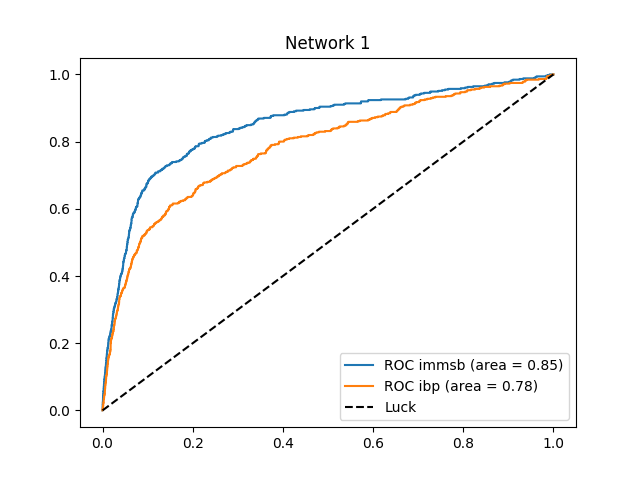
\includegraphics[width=\textwidth]{img/corpus/roc_network1}
            \label{fig:mean and std of net14}
            \caption {{\small Network1}}    
        \end{subfigure}
        \begin{subfigure}[b]{0.300\textwidth}
            \centering
            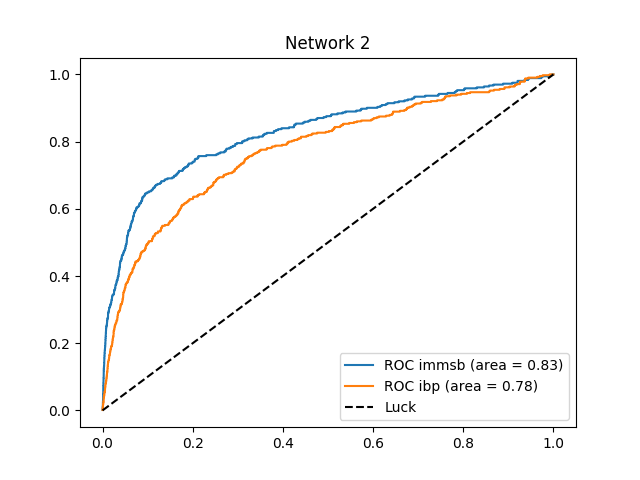
\includegraphics[width=\textwidth]{img/corpus/roc_network2}
            \label{fig:mean and std of net14}
            \caption {{\small Network2}}    
        \end{subfigure}
        \begin{subfigure}[b]{0.300\textwidth}
            \centering
            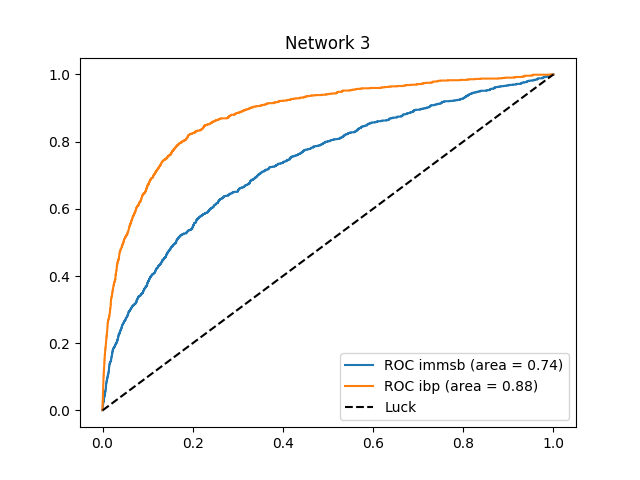
\includegraphics[width=\textwidth]{img/corpus/roc_network3}
            \label{fig:mean and std of net14}
            \caption {{\small Network3}}    
        \end{subfigure}
        \begin{subfigure}[b]{0.300\textwidth}
            \centering
            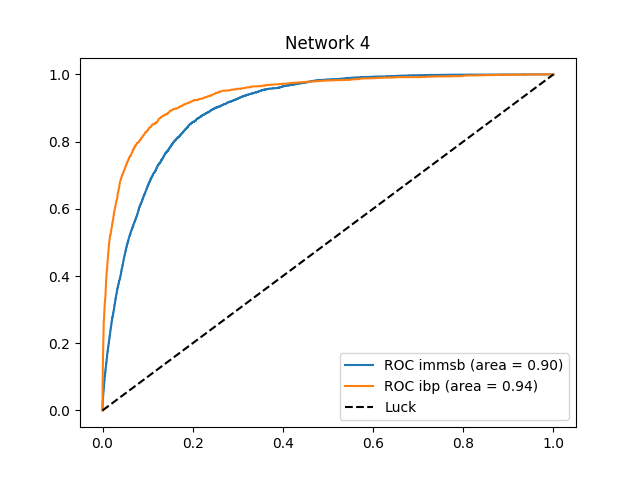
\includegraphics[width=\textwidth]{img/corpus/roc_network4}
            \label{fig:mean and std of net14}
            \caption {{\small Network4}}    
        \end{subfigure}
        \begin{subfigure}[b]{0.300\textwidth}
            \centering
            \includegraphics[width=\textwidth]{img/corpus/roc_manufacturing}
            \label{fig:mean and std of net14}
            \caption {{\small Manufacturing}}    
        \end{subfigure}
        \begin{subfigure}[b]{0.300\textwidth}
            \centering
            \includegraphics[width=\textwidth]{img/corpus/roc_ucirvine}
            \label{fig:mean and std of net14}
            \caption {{\small Manufacturing}}    
        \end{subfigure}
        \begin{subfigure}[b]{0.300\textwidth}
            \centering
            \includegraphics[width=\textwidth]{img/corpus/roc_blogs}
            \caption {{\small Blogs}}    
            \label{fig:mean and std of net14}
        \end{subfigure}
        \begin{subfigure}[b]{0.300\textwidth}
            \centering
            \includegraphics[width=\textwidth]{img/corpus/roc_emaileu}
            \caption {{\small Email Europe}}    
            \label{fig:mean and std of net14}
        \end{subfigure}
        \begin{subfigure}[b]{0.300\textwidth}
            \centering
            \includegraphics[width=\textwidth]{img/corpus/roc_protein}
            \caption {{\small Protein}}    
            \label{fig:mean and std of net14}
        \end{subfigure}
        %\quad
        %\hfill
	\caption{AUC curves that compare the performance of ILFM and IMMSB on the 4 synthetic networks.}
	\label{fig:auc}
\end{figure}


\subsubsection{Comments}
\textcolor{red}{here comment...} 

\section{$M_e$ -- Model Generated}
\label{sec:mgmg}

\subsection{Burstiness}

\textcolor{red}{Je changerais la forme (comment les groupe de figure sont plotté) selon ce que lon conviendra de conserver dan le partie expé.}

We illustrate the burstiness results by generating 3 random networks for each of both models. We report it in figure \ref{fig:gen_burst}. We use the 3 same settings for IMMSB  than those in the previous section. For ILFM  we use the following 3 settings: (column 1:$\alpha=1,  \lambda_1=\lambda_2=1$ , column 2:$\alpha=0.1, \lambda_1=\lambda_2=1$, column 3: $\alpha=1, \lambda_1=\lambda_2=10$) and we fix $\sigma_w=1$ and again $N=1000$.

Each row of the two sets of figures represents the three following measures who corresponds respectively to the global preferential attachment, the local preferential attachment and the feature burstiness:
\begin{itemize}
    \item First row: we measure the overall degree distributions; We report the average and standard deviation of the degree distribution in a linear scale for each generated network.
    \item Second row: we measure the local degree distribution on a log-log scale:
        \begin{itemize}
            \item for IMMSB, each network has an associated membership tensor $Z$, that indicates the membership of nodes for each  interactions. In order to draw the local degree distribution for a block $c$, we reduce the adjacency matrix in order to retain only the links that occurs inside a block $c$. The local degree distribution is thus computed on the reduce adjacency matrix $Y_c = Y \otimes (Z_i^c \times Z_j^c)$ where $\otimes$ is the hadamard product and $\times$ the outer product. $Z_i^c$ is the membership matrix of a nodes $i$ such that $Z_{ik}^c=0$ if $k\neq c$ (links that occurs outside $c$ will be ignored).
            \item for ILFM, each node is associated with a fix feature vector; the local degree distribution for the block $c$ is obtain by taking only the contribution of the features $c$ on the adjacency matrix. Thus, the local degree degree distribution is computed on the reduce adjacency matrix $Y_c = Y \otimes (F_{.c}\times F_{.c})$. 
        \end{itemize}
    \item Third row measure the distribution of the block membership, which directly reflect the feature burstiness. Hence for IMMSB, for a feature $k$, we measure $\sum_{ij} \mathds{1}(Z_{i\rightarrow j} = k, Z_{i\leftarrow j} = k)$ which indicates the number of nodes who were associated to the block $k$. For ILFM the number of nodes associated to a block $k$ is simply $\sum_n F_{nk}$.
\end{itemize}


% not sure it use significantly usefull, because p-value are either 0 or 1 ...
%We provide in annexe (\textcolor{red}{not yet included}),  an goodness of fit for all local degrees distribution that we plotted, in order to quantify the power law hypothesis on the empirical degree distributions. The number of feature is typically too small to evaluate an significant goodness of fit. The protocol is described in section \ref{sec:experiments-busrt}. 

The simulation shows us the following facts about the properties of the models:
\begin{itemize}
	\item For both model the global degree distribution don't exhibit a bursty phenomenon,
	\item The local degree distribution show that IMMSB exhibit a bursty phenomenon which is not the case for ILFM,
	\item Both models exhibits a bursty phenomenon on the feature distribution. This distributions for ILFM has a long tail for all of the 3 settings while for IMMSB, the tail shape is more or less long depending of the $\alpha$ and $\gamma$ parameters.
\end{itemize}

For the case of the global preferential attachment we have no formal proof for the non-compliance of the models, due the non closed form of the evidence in both models, due to the admixture design \textcolor{red}{ref ((Multiple Hypergeometric Functions: Probabilistic Interpretations and Statistical Uses
James M. Dickey )) ce papier est cite dans LDA pour justifier l'inference approxime, mais je n'arrive pas a trouver ca papier !!!}. However, as reported simulations (figure \ref{fig:gen_burst}), we see that the empirical distributions of the overall degrees are clearly non bursty.

%
\begin{figure}[ht]
    \vspace{-3cm}
	\centering IMMSB\\
	\minipage{0.27\textwidth}
	\includegraphics[scale=0.27]{img/M_g_peaks/figure_1}
	\endminipage
		\minipage{0.27\textwidth}
	\includegraphics[scale=0.27]{img/M_g_power_law/figure_1}
	\endminipage
	\minipage{0.27\textwidth}
	\includegraphics[scale=0.27]{img/M_g_regular/figure_1}
	\endminipage
		\vspace{-0.29cm}
	\minipage{0.27\textwidth}
	\includegraphics[scale=0.27]{img/M_g_peaks/figure_3}
	\endminipage
		\minipage{0.27\textwidth}
	\includegraphics[scale=0.27]{img/M_g_power_law/figure_3} 
	\endminipage
	\minipage{0.27\textwidth}
	\includegraphics[scale=0.27]{img/M_g_regular/figure_3}
	\endminipage
		\vspace{-0.28cm}
	\minipage{0.27\textwidth}
	\includegraphics[scale=0.27]{img/M_g_peaks/figure_5}
	\endminipage
	\minipage{0.27\textwidth}
	\includegraphics[scale=0.27]{img/M_g_power_law/figure_5} 
	\endminipage
	\minipage{0.27\textwidth}
	\includegraphics[scale=0.27]{img/M_g_regular/figure_5}
	\endminipage

    \vspace{0.2cm}
	 ILFM

	\minipage{0.27\textwidth}
	\includegraphics[scale=0.27]{img/ilfm/1/figure_1}
	\endminipage
		\minipage{0.27\textwidth}
	\includegraphics[scale=0.27]{img/ilfm/2/figure_1}
	\endminipage
	\minipage{0.27\textwidth}
	\includegraphics[scale=0.27]{img/ilfm/3/figure_1}
	\endminipage
		\vspace{-0.29cm}
	\minipage{0.27\textwidth}
	\includegraphics[scale=0.27]{img/ilfm/1/figure_3}
	\endminipage
		\minipage{0.27\textwidth}
	\includegraphics[scale=0.27]{img/ilfm/2/figure_3} 
	\endminipage
	\minipage{0.27\textwidth}
	\includegraphics[scale=0.27]{img/ilfm/3/figure_3}
	\endminipage
		\vspace{-0.28cm}
	\minipage{0.27\textwidth}
	\includegraphics[scale=0.27]{img/ilfm/1/figure_5}
	\endminipage
	\minipage{0.27\textwidth}
	\includegraphics[scale=0.27]{img/ilfm/2/figure_5} 
	\endminipage
	\minipage{0.27\textwidth}
	\includegraphics[scale=0.27]{img/ilfm/3/figure_5}
	\endminipage
    \caption{\tiny{Generated Networks with IMMSB (top) and ILFM (bottom) for three different settings (same set than for figure \ref{fig:gen_blocks_mmsb}). The top rows measure the global preferential attachment through the overall degree distribution. The middle row measure the local preferential attachment through the local degree distribution. The last row measure the feature burstiness through the block membership distribution.}}
	\label{fig:gen_burst}
\end{figure}



\subsection{Homophily}


\bibliographystyle{unsrt}
\bibliography{./a}

\end{document}
